
%% bare_jrnl.tex
%% V1.4b
%% 2015/08/26
%% by Michael Shell
%% see http://www.michaelshell.org/
%% for current contact information.
%%
%% This is a skeleton file demonstrating the use of IEEEtran.cls
%% (requires IEEEtran.cls version 1.8b or later) with an IEEE
%% journal paper.
%%
%% Support sites:
%% http://www.michaelshell.org/tex/ieeetran/
%% http://www.ctan.org/pkg/ieeetran
%% and
%% http://www.ieee.org/

%%*************************************************************************
%% Legal Notice:
%% This code is offered as-is without any warranty either expressed or
%% implied; without even the implied warranty of MERCHANTABILITY or
%% FITNESS FOR A PARTICULAR PURPOSE!
%% User assumes all risk.
%% In no event shall the IEEE or any contributor to this code be liable for
%% any damages or losses, including, but not limited to, incidental,
%% consequential, or any other damages, resulting from the use or misuse
%% of any information contained here.
%%
%% All comments are the opinions of their respective authors and are not
%% necessarily endorsed by the IEEE.
%%
%% This work is distributed under the LaTeX Project Public License (LPPL)
%% ( http://www.latex-project.org/ ) version 1.3, and may be freely used,
%% distributed and modified. A copy of the LPPL, version 1.3, is included
%% in the base LaTeX documentation of all distributions of LaTeX released
%% 2003/12/01 or later.
%% Retain all contribution notices and credits.
%% ** Modified files should be clearly indicated as such, including  **
%% ** renaming them and changing author support contact information. **
%%*************************************************************************


% *** Authors should verify (and, if needed, correct) their LaTeX system  ***
% *** with the testflow diagnostic prior to trusting their LaTeX platform ***
% *** with production work. The IEEE's font choices and paper sizes can   ***
% *** trigger bugs that do not appear when using other class files.       ***                          ***
% The testflow support page is at:
% http://www.michaelshell.org/tex/testflow/



\documentclass[journal]{IEEEtran}
%
% If IEEEtran.cls has not been installed into the LaTeX system files,
% manually specify the path to it like:
% \documentclass[journal]{../sty/IEEEtran}





% Some very useful LaTeX packages include:
% (uncomment the ones you want to load)


% *** MISC UTILITY PACKAGES ***
%
%\usepackage{ifpdf}
% Heiko Oberdiek's ifpdf.sty is very useful if you need conditional
% compilation based on whether the output is pdf or dvi.
% usage:
% \ifpdf
%   % pdf code
% \else
%   % dvi code
% \fi
% The latest version of ifpdf.sty can be obtained from:
% http://www.ctan.org/pkg/ifpdf
% Also, note that IEEEtran.cls V1.7 and later provides a builtin
% \ifCLASSINFOpdf conditional that works the same way.
% When switching from latex to pdflatex and vice-versa, the compiler may
% have to be run twice to clear warning/error messages.






% *** CITATION PACKAGES ***
%
%\usepackage{cite}
% cite.sty was written by Donald Arseneau
% V1.6 and later of IEEEtran pre-defines the format of the cite.sty package
% \cite{} output to follow that of the IEEE. Loading the cite package will
% result in citation numbers being automatically sorted and properly
% "compressed/ranged". e.g., [1], [9], [2], [7], [5], [6] without using
% cite.sty will become [1], [2], [5]--[7], [9] using cite.sty. cite.sty's
% \cite will automatically add leading space, if needed. Use cite.sty's
% noadjust option (cite.sty V3.8 and later) if you want to turn this off
% such as if a citation ever needs to be enclosed in parenthesis.
% cite.sty is already installed on most LaTeX systems. Be sure and use
% version 5.0 (2009-03-20) and later if using hyperref.sty.
% The latest version can be obtained at:
% http://www.ctan.org/pkg/cite
% The documentation is contained in the cite.sty file itself.






% *** GRAPHICS RELATED PACKAGES ***
%
\ifCLASSINFOpdf
  % \usepackage[pdftex]{graphicx}
  % declare the path(s) where your graphic files are
  % \graphicspath{{../pdf/}{../jpeg/}}
  % and their extensions so you won't have to specify these with
  % every instance of \includegraphics
  % \DeclareGraphicsExtensions{.pdf,.jpeg,.png}
\else
  % or other class option (dvipsone, dvipdf, if not using dvips). graphicx
  % will default to the driver specified in the system graphics.cfg if no
  % driver is specified.
  % \usepackage[dvips]{graphicx}
  % declare the path(s) where your graphic files are
  % \graphicspath{{../eps/}}
  % and their extensions so you won't have to specify these with
  % every instance of \includegraphics
  % \DeclareGraphicsExtensions{.eps}
\fi
% graphicx was written by David Carlisle and Sebastian Rahtz. It is
% required if you want graphics, photos, etc. graphicx.sty is already
% installed on most LaTeX systems. The latest version and documentation
% can be obtained at:
% http://www.ctan.org/pkg/graphicx
% Another good source of documentation is "Using Imported Graphics in
% LaTeX2e" by Keith Reckdahl which can be found at:
% http://www.ctan.org/pkg/epslatex
%
% latex, and pdflatex in dvi mode, support graphics in encapsulated
% postscript (.eps) format. pdflatex in pdf mode supports graphics
% in .pdf, .jpeg, .png and .mps (metapost) formats. Users should ensure
% that all non-photo figures use a vector format (.eps, .pdf, .mps) and
% not a bitmapped formats (.jpeg, .png). The IEEE frowns on bitmapped formats
% which can result in "jaggedy"/blurry rendering of lines and letters as
% well as large increases in file sizes.
%
% You can find documentation about the pdfTeX application at:
% http://www.tug.org/applications/pdftex





% *** MATH PACKAGES ***
%
\usepackage{amsmath,amssymb}
\usepackage{amsthm}
\newtheorem{theorem}{Theorem}
\newtheorem*{cor}{Corollary}
\newtheorem{lemma}[theorem]{Lemma}
\DeclareMathOperator\erfc{erfc}
\DeclareMathOperator\erf{erf}
% A popular package from the American Mathematical Society that provides
% many useful and powerful commands for dealing with mathematics.
%
% Note that the amsmath package sets \interdisplaylinepenalty to 10000
% thus preventing page breaks from occurring within multiline equations. Use:
%\interdisplaylinepenalty=2500
% after loading amsmath to restore such page breaks as IEEEtran.cls normally
% does. amsmath.sty is already installed on most LaTeX systems. The latest
% version and documentation can be obtained at:
% http://www.ctan.org/pkg/amsmath





% *** SPECIALIZED LIST PACKAGES ***
%
%\usepackage{algorithmic}
% algorithmic.sty was written by Peter Williams and Rogerio Brito.
% This package provides an algorithmic environment fo describing algorithms.
% You can use the algorithmic environment in-text or within a figure
% environment to provide for a floating algorithm. Do NOT use the algorithm
% floating environment provided by algorithm.sty (by the same authors) or
% algorithm2e.sty (by Christophe Fiorio) as the IEEE does not use dedicated
% algorithm float types and packages that provide these will not provide
% correct IEEE style captions. The latest version and documentation of
% algorithmic.sty can be obtained at:
% http://www.ctan.org/pkg/algorithms
% Also of interest may be the (relatively newer and more customizable)
% algorithmicx.sty package by Szasz Janos:
% http://www.ctan.org/pkg/algorithmicx




% *** ALIGNMENT PACKAGES ***
%
%\usepackage{array}
% Frank Mittelbach's and David Carlisle's array.sty patches and improves
% the standard LaTeX2e array and tabular environments to provide better
% appearance and additional user controls. As the default LaTeX2e table
% generation code is lacking to the point of almost being broken with
% respect to the quality of the end results, all users are strongly
% advised to use an enhanced (at the very least that provided by array.sty)
% set of table tools. array.sty is already installed on most systems. The
% latest version and documentation can be obtained at:
% http://www.ctan.org/pkg/array


% IEEEtran contains the IEEEeqnarray family of commands that can be used to
% generate multiline equations as well as matrices, tables, etc., of high
% quality.




% *** SUBFIGURE PACKAGES ***
%\ifCLASSOPTIONcompsoc
%  \usepackage[caption=false,font=normalsize,labelfont=sf,textfont=sf]{subfig}
%\else
%  \usepackage[caption=false,font=footnotesize]{subfig}
%\fi
% subfig.sty, written by Steven Douglas Cochran, is the modern replacement
% for subfigure.sty, the latter of which is no longer maintained and is
% incompatible with some LaTeX packages including fixltx2e. However,
% subfig.sty requires and automatically loads Axel Sommerfeldt's caption.sty
% which will override IEEEtran.cls' handling of captions and this will result
% in non-IEEE style figure/table captions. To prevent this problem, be sure
% and invoke subfig.sty's "caption=false" package option (available since
% subfig.sty version 1.3, 2005/06/28) as this is will preserve IEEEtran.cls
% handling of captions.
% Note that the Computer Society format requires a larger sans serif font
% than the serif footnote size font used in traditional IEEE formatting
% and thus the need to invoke different subfig.sty package options depending
% on whether compsoc mode has been enabled.
%
% The latest version and documentation of subfig.sty can be obtained at:
% http://www.ctan.org/pkg/subfig




% *** FLOAT PACKAGES ***
%
%\usepackage{fixltx2e}
% fixltx2e, the successor to the earlier fix2col.sty, was written by
% Frank Mittelbach and David Carlisle. This package corrects a few problems
% in the LaTeX2e kernel, the most notable of which is that in current
% LaTeX2e releases, the ordering of single and double column floats is not
% guaranteed to be preserved. Thus, an unpatched LaTeX2e can allow a
% single column figure to be placed prior to an earlier double column
% figure.
% Be aware that LaTeX2e kernels dated 2015 and later have fixltx2e.sty's
% corrections already built into the system in which case a warning will
% be issued if an attempt is made to load fixltx2e.sty as it is no longer
% needed.
% The latest version and documentation can be found at:
% http://www.ctan.org/pkg/fixltx2e


%\usepackage{stfloats}
% stfloats.sty was written by Sigitas Tolusis. This package gives LaTeX2e
% the ability to do double column floats at the bottom of the page as well
% as the top. (e.g., "\begin{figure*}[!b]" is not normally possible in
% LaTeX2e). It also provides a command:
%\fnbelowfloat
% to enable the placement of footnotes below bottom floats (the standard
% LaTeX2e kernel puts them above bottom floats). This is an invasive package
% which rewrites many portions of the LaTeX2e float routines. It may not work
% with other packages that modify the LaTeX2e float routines. The latest
% version and documentation can be obtained at:
% http://www.ctan.org/pkg/stfloats
% Do not use the stfloats baselinefloat ability as the IEEE does not allow
% \baselineskip to stretch. Authors submitting work to the IEEE should note
% that the IEEE rarely uses double column equations and that authors should try
% to avoid such use. Do not be tempted to use the cuted.sty or midfloat.sty
% packages (also by Sigitas Tolusis) as the IEEE does not format its papers in
% such ways.
% Do not attempt to use stfloats with fixltx2e as they are incompatible.
% Instead, use Morten Hogholm'a dblfloatfix which combines the features
% of both fixltx2e and stfloats:
%
% \usepackage{dblfloatfix}
% The latest version can be found at:
% http://www.ctan.org/pkg/dblfloatfix




%\ifCLASSOPTIONcaptionsoff
%  \usepackage[nomarkers]{endfloat}
% \let\MYoriglatexcaption\caption
% \renewcommand{\caption}[2][\relax]{\MYoriglatexcaption[#2]{#2}}
%\fi
% endfloat.sty was written by James Darrell McCauley, Jeff Goldberg and
% Axel Sommerfeldt. This package may be useful when used in conjunction with
% IEEEtran.cls'  captionsoff option. Some IEEE journals/societies require that
% submissions have lists of figures/tables at the end of the paper and that
% figures/tables without any captions are placed on a page by themselves at
% the end of the document. If needed, the draftcls IEEEtran class option or
% \CLASSINPUTbaselinestretch interface can be used to increase the line
% spacing as well. Be sure and use the nomarkers option of endfloat to
% prevent endfloat from "marking" where the figures would have been placed
% in the text. The two hack lines of code above are a slight modification of
% that suggested by in the endfloat docs (section 8.4.1) to ensure that
% the full captions always appear in the list of figures/tables - even if
% the user used the short optional argument of \caption[]{}.
% IEEE papers do not typically make use of \caption[]'s optional argument,
% so this should not be an issue. A similar trick can be used to disable
% captions of packages such as subfig.sty that lack options to turn off
% the subcaptions:
% For subfig.sty:
% \let\MYorigsubfloat\subfloat
% \renewcommand{\subfloat}[2][\relax]{\MYorigsubfloat[]{#2}}
% However, the above trick will not work if both optional arguments of
% the \subfloat command are used. Furthermore, there needs to be a
% description of each subfigure *somewhere* and endfloat does not add
% subfigure captions to its list of figures. Thus, the best approach is to
% avoid the use of subfigure captions (many IEEE journals avoid them anyway)
% and instead reference/explain all the subfigures within the main caption.
% The latest version of endfloat.sty and its documentation can obtained at:
% http://www.ctan.org/pkg/endfloat
%
% The IEEEtran \ifCLASSOPTIONcaptionsoff conditional can also be used
% later in the document, say, to conditionally put the References on a
% page by themselves.




% *** PDF, URL AND HYPERLINK PACKAGES ***
%
%\usepackage{url}
% url.sty was written by Donald Arseneau. It provides better support for
% handling and breaking URLs. url.sty is already installed on most LaTeX
% systems. The latest version and documentation can be obtained at:
% http://www.ctan.org/pkg/url
% Basically, \url{my_url_here}.




% *** Do not adjust lengths that control margins, column widths, etc. ***
% *** Do not use packages that alter fonts (such as pslatex).         ***
% There should be no need to do such things with IEEEtran.cls V1.6 and later.
% (Unless specifically asked to do so by the journal or conference you plan
% to submit to, of course. )


% correct bad hyphenation here
\hyphenation{op-tical net-works semi-conduc-tor}


\begin{document}

% !TEX root = ../partial-sdm.tex

%
% paper title
% Titles are generally capitalized except for words such as a, an, and, as,
% at, but, by, for, in, nor, of, on, or, the, to and up, which are usually
% not capitalized unless they are the first or last word of the title.
% Linebreaks \\ can be used within to get better formatting as desired.
% Do not put math or special symbols in the title.
\title{Autocorrelation in Sparse Distributed Memory}
%
%
% author names and IEEE memberships
% note positions of commas and nonbreaking spaces ( ~ ) LaTeX will not break
% a structure at a ~ so this keeps an author's name from being broken across
% two lines.
% use \thanks{} to gain access to the first footnote area
% a separate \thanks must be used for each paragraph as LaTeX2e's \thanks
% was not built to handle multiple paragraphs
%

\author{Marcelo S. Brogliato,~\IEEEmembership{Member,~IEEE,}
        and~Alexandre Linhares,~\IEEEmembership{Member,~IEEE}% <-this % stops a space
\thanks{M. Brogliato was with the Department
of Electrical and Computer Engineering, Georgia Institute of Technology, Atlanta,
GA, 30332 USA e-mail: (see http://www.michaelshell.org/contact.html).}% <-this % stops a space
\thanks{J. Doe and J. Doe are with Anonymous University.}% <-this % stops a space
\thanks{Manuscript received April 19, 2005; revised August 26, 2015.}}

% note the % following the last \IEEEmembership and also \thanks -
% these prevent an unwanted space from occurring between the last author name
% and the end of the author line. i.e., if you had this:
%
% \author{....lastname \thanks{...} \thanks{...} }
%                     ^------------^------------^----Do not want these spaces!
%
% a space would be appended to the last name and could cause every name on that
% line to be shifted left slightly. This is one of those "LaTeX things". For
% instance, "\textbf{A} \textbf{B}" will typeset as "A B" not "AB". To get
% "AB" then you have to do: "\textbf{A}\textbf{B}"
% \thanks is no different in this regard, so shield the last } of each \thanks
% that ends a line with a % and do not let a space in before the next \thanks.
% Spaces after \IEEEmembership other than the last one are OK (and needed) as
% you are supposed to have spaces between the names. For what it is worth,
% this is a minor point as most people would not even notice if the said evil
% space somehow managed to creep in.



% The paper headers
\markboth{Journal of \LaTeX\ Class Files,~Vol.~14, No.~8, August~2015}%
{Shell \MakeLowercase{\textit{et al.}}: Bare Demo of IEEEtran.cls for IEEE Journals}
% The only time the second header will appear is for the odd numbered pages
% after the title page when using the twoside option.
%
% *** Note that you probably will NOT want to include the author's ***
% *** name in the headers of peer review papers.                   ***
% You can use \ifCLASSOPTIONpeerreview for conditional compilation here if
% you desire.




% If you want to put a publisher's ID mark on the page you can do it like
% this:
%\IEEEpubid{0000--0000/00\$00.00~\copyright~2015 IEEE}
% Remember, if you use this you must call \IEEEpubidadjcol in the second
% column for its text to clear the IEEEpubid mark.



% use for special paper notices
%\IEEEspecialpapernotice{(Invited Paper)}




% make the title area
\maketitle

% As a general rule, do not put math, special symbols or citations
% in the abstract or keywords.
\begin{abstract}
The abstract goes here.
\end{abstract}

% Note that keywords are not normally used for peerreview papers.
\begin{IEEEkeywords}
IEEE, IEEEtran, journal, \LaTeX, paper, template.
\end{IEEEkeywords}






% For peer review papers, you can put extra information on the cover
% page as needed:
% \ifCLASSOPTIONpeerreview
% \begin{center} \bfseries EDICS Category: 3-BBND \end{center}
% \fi
%
% For peerreview papers, this IEEEtran command inserts a page break and
% creates the second title. It will be ignored for other modes.
\IEEEpeerreviewmaketitle



\section{Introduction}

%% !TEX root = ../partial-sdm.tex

\section{A deviation from the equator distance?}

Kanerva writes\footnote{Email thread `SDM: A puzzling issue and an invitation', started March 16th 2018, in which we discussed the aforementioned discrepancy.  To think that some centuries ago, all scientific publishing was the exchange of such letters.}:

\begin{quote}
    You have done an incredibly thorough analysis of SDM. I like the puzzle in your message and believe that your simulations are correct and to be learned from.  So what to make of the difference compared to my Figure 7.3 (and your Figure \ref{fig:kanerva-figure-73-calculated})?  I think the difference comes from my not having accounted fully for the effect of the other 9,999 vectors that are stored in the memory.  You say in it\\

   ``Our results show that the theoretical prediction is not accurate. There are interaction effects from one or more of the attractors created by the 10,000 writes, and these attractors seem to raise the distance beyond 500 bits (Figure \ref{fig:sdm-10000w-table-7-2}).'' \\

   I think that is correct.  It also brings to mind a comment Louis Jaeckel made when we worked at NASA Ames.  He pointed out that autoassociative storage (each vector is stored with itself as the address) introduces autocorrelation that my formula for Figure 7.2 did not take into account.  When we read from memory, each stored vector exerts a pull toward itself, which also means that each bit of a retrieved vector is slightly biased toward the same bit of the read address, regardless of the read address.  We never worked out the math.
\end{quote}

This is an important observation. A hard location is activated because it shares many dimensions with the items read from or written onto it. Imagine the `counter's eye view':  each individual counter `likes'\footnote{If you are a cell I then I have some serious piece of advice to you.  I would strongly suggest avoiding the neighborhood of a neuron. Neurons have serious authoritarian tendencies, bossing around --- generally electrifying --- the hopeless innocent cells around them just because.} to write on its own corresponding bit-address value more than it likes the opposite; as each hard-location has a say in its own area --- and nowhere else.

Let $x$ and $y$ be random bitstrings and $n$ be the number of dimensions in the memory; let $x_i$ and $y_i$ be the $i$-th bit of $x$ and $y$, respectively; and $d(x, y)$ be the Hamming distance. Whilst the probability of a shared bit-value between same dimension-bits in two random addresses is $1/2$, an address only activates hard-locations close to it.  Let us call these shared bitvalues a \emph{bitmatch in dimension $i$}.

So, what is the probability of bitmatches given that we know the access radius $r$ between the address and a hard-location?
\bigskip

\begin{theorem}
\emph{Each dimension has a small pull bias, which can be measured by}
\label{T1}
$P(x_i = y_i | d(x, y) \le r) = \dfrac{\sum_{k=0}^{r} \binom{n-1}{k}}{\sum_{k=0}^{r} \binom{n}{k}}.$
\end{theorem}

\begin{proof}
    The left-hand expression $P(x_i = y_i | d(x, y) \le r)$ computes the probability of a bitmatch in $i$, given that we know that $x$ and $y$ are in the access radius defined by $r$, i.e., $d(x, y)\le r$.

    Applying the law of total probability to the left-hand expression we obtain

    \begin{align}
    \sum_{k=0}^{r} P(x_i = y_i | d(x, y) = k \le r) P(d(x, y) = k | d(x, y) \le r)
    \end{align}

    We also know that

    \begin{align}
    P(x_i = y_i | d(x, y) = k) &= \frac{n-k}{n} \\
    P(d(x, y) = k | d(x, y) \le r) &= \frac{\binom{n}{k}}{\sum_{j=0}^{r} \binom{n}{j}}
    \end{align}

    Hence,

    \begin{align}
    P(x_i = y_i | d(x, y) \le r) = \frac{\sum_{k=0}^{r} \frac{n-k}{n} \binom{n}{k}}{\sum_{j=0}^{r} \binom{n}{j}}
    \end{align}

    Finally, the combinatorial identity

    \begin{align}
    \frac{n-k}{n} \binom{n}{k} = \frac{(n-k)}{n} \frac{n!}{(n-k)! k!} = \frac{(n-1)!}{k! (n-1-k)!} = \binom{n-1}{k}
    \end{align}

    closes the theorem.

\end{proof}

Theorem \ref{T1} is valid for both ``x written at x'' (autoassociative memory) and ``random written at x'' (heteroassociative memory). When $n=1,000$ and $r=451$, $P(x_i = y_i | d(x, y) \le r) = p = 0.552905498137$.  Each bit of a hard location does indeed have a small pull bias.  What is meant by this is that each particular dimension has a small preference toward positive values if its address bit is set to 1, and negative values if set to 0.


\begin{lemma}
Let $r$ be the access radius given that $f$ percent of the hard locations are activated. Then, $\lim_{n \rightarrow \infty} r/n = 1/2$.
\label{thm:sdm-access-radius}
\end{lemma}
\begin{proof}

As the bits of the hard locations' addresses are randomly chosen, the distance between two hard locations follow a Binomial distribution with $n$ samples and probability 0.5 ($B(n, 0.5)$). For $n$ sufficiently large, the Binomial distribution can be approximated by a Normal distribution, i.e., $B(n, 0.5) \rightarrow \mathcal{N}(\mu = n/2, \sigma^2 = n/4)$.

Let $\Phi(x)$ be the cdf of the standard normal distribution. Let $z = \frac{r - n/2}{\sqrt{n}/2}$. Thus, $P(d(x, y) \le r) = \Phi(z)$. As $f = P(d(x, y) \le r)$, then, $f = \Phi(z)$.

Calculating the inverse, $z = \Phi^{-1}(f)$. Then,

\begin{align}
z &= \Phi^{-1}(f) \\
\frac{r - n/2}{\sqrt{n}/2} &= \Phi^{-1}(f) \\
r &= \frac{n}{2} + \Phi^{-1}(f) \frac{\sqrt{n}}{2} \\
\frac{r}{n} &= \frac{1}{2} + \Phi^{-1}(f) \frac{1}{2 \sqrt{n}}
\end{align}

Therefore, $n \rightarrow \infty \Rightarrow r/n \rightarrow 1/2$.
\end{proof}

\begin{lemma}
Let $\Phi(x)$ be the cdf of the standard normal distribution. Then, $n \rightarrow \infty \Rightarrow P(x_i = y_i | d(x, y) \le r) = \frac{1}{2} \frac{\Phi(z_1)}{\Phi(z_2)}$, where $z_1 = \frac{2r - n + 1}{\sqrt{n-1}}$ and $z_2 = \frac{2r - n}{\sqrt{n}}$.
\label{thm:sdm-T1-n-large}
\end{lemma}
\begin{proof}

From the approximation of the Binomial distribution $B(a, 0.5)$ by the Normal distribution $\mathcal{N}(\mu = a/2, \sigma^2 = a/4)$, we conclude that, for $a$ sufficiently large, the cdf of the Binomial is approximately equal to the cdf of the Normal distribution. Thus,

$$
\frac{1}{2^a} \sum_{k=0}^{b} \binom{a}{k} = \Phi \left( \frac{b-a/2}{\sqrt{a}/2} \right) = \Phi \left( \frac{2b-a}{\sqrt{a}} \right)
$$

Thus,

$$
\sum_{k=0}^{b} \binom{a}{k} = 2^a \Phi \left( \frac{2b-a}{\sqrt{a}} \right)
$$

The result comes directly from applyting the equation above in $P(x_i = y_i | d(x, y) \le r)$.

\end{proof}

\begin{theorem}
The autocorrelation vanishes when $n \rightarrow \infty$, i.e., $\lim_{n \rightarrow \infty} P(x_i = y_i | d(x, y) \le r) = 1/2$.
\label{thm:sdm-autocorrelation-convergence}
\end{theorem}
\begin{proof}

From Lemma \ref{thm:sdm-access-radius}, we know that $r = n/2$ for $n$ sufficiently large. Thus, replacing $r = n/2$ in Lemma \ref{thm:sdm-T1-n-large}, $P(x_i = y_i | d(x, y) \le r) = \frac{\Phi(z_1)}{2 \Phi(z_2)}$, where $z_1 = \frac{1}{\sqrt{n-1}}$ and $z_2 = 0$.

As $n \rightarrow \infty$, $z_1 \rightarrow 0$, and $P(x_i = y_i | d(x, y) \le r) = \frac{\Phi(0)}{2 \Phi(0)} = 1/2$. \qed

Another way to proof is to divide into two cases:

Suppose that $n$ is an even integer, then,

$$
\sum_{k=0}^{r} \binom{n}{k} = \sum_{k=0}^{n/2} \binom{n}{k} = \frac{1}{2} \sum_{k=0}^{n} \binom{n}{k} = \frac{2^n}{2} = 2^{n-1}
$$

And, also,

\begin{align*}
\sum_{k=0}^{r} \binom{n-1}{k} &= \sum_{k=0}^{n/2} \binom{n-1}{k} \\
    &= \frac{1}{2} \left[ \sum_{k=0}^{n-1} \binom{n-1}{k} - \binom{n-1}{n/2} \right] \\
    &= \frac{1}{2} \left[ 2^{n-1} - \binom{n-1}{n/2} \right] \\
    &= 2^{n-2} - \frac{1}{2} \binom{n-1}{n/2}
\end{align*}

Finally,

\begin{align}
P(x_i = y_i | d(x, y) \le r) &= \frac{\sum_{k=0}^{r} \binom{n-1}{k}}{\sum_{k=0}^{r} \binom{n}{k}} \\
    &= \frac{2^{n-2} - \frac{1}{2} \binom{n-1}{n/2}}{2^{n-1}} \\
    &= \frac{2^{n-2}}{2^{n-1}} - \frac{1}{2^n} \binom{n-1}{n/2} \\
    &= \frac{1}{2} - \frac{1}{2^n} \binom{n-1}{n/2}
\end{align}

As $n \rightarrow \infty \Rightarrow \frac{1}{2^n} \binom{n-1}{n/2} \rightarrow 0$, the proof is done for $n$ even.

When $n$ is an odd integer, the steps of the proof are similar. Therefore, the proof is complete.

\end{proof}

In Figure \ref{fig:sdm-10kbits-figure-7-3}, with $n=10,000$ and $r=4,845$, we can notice that the autocorrelation has reduced significantly as predicted by Theorem \ref{thm:sdm-autocorrelation-convergence}. In fact, in this case, using Lemma \ref{thm:sdm-T1-n-large}, $P(x_i = y_i | d(x, y) \le r) = 0.5168761116022098$.

\begin{figure}[!htb]
  \centering
  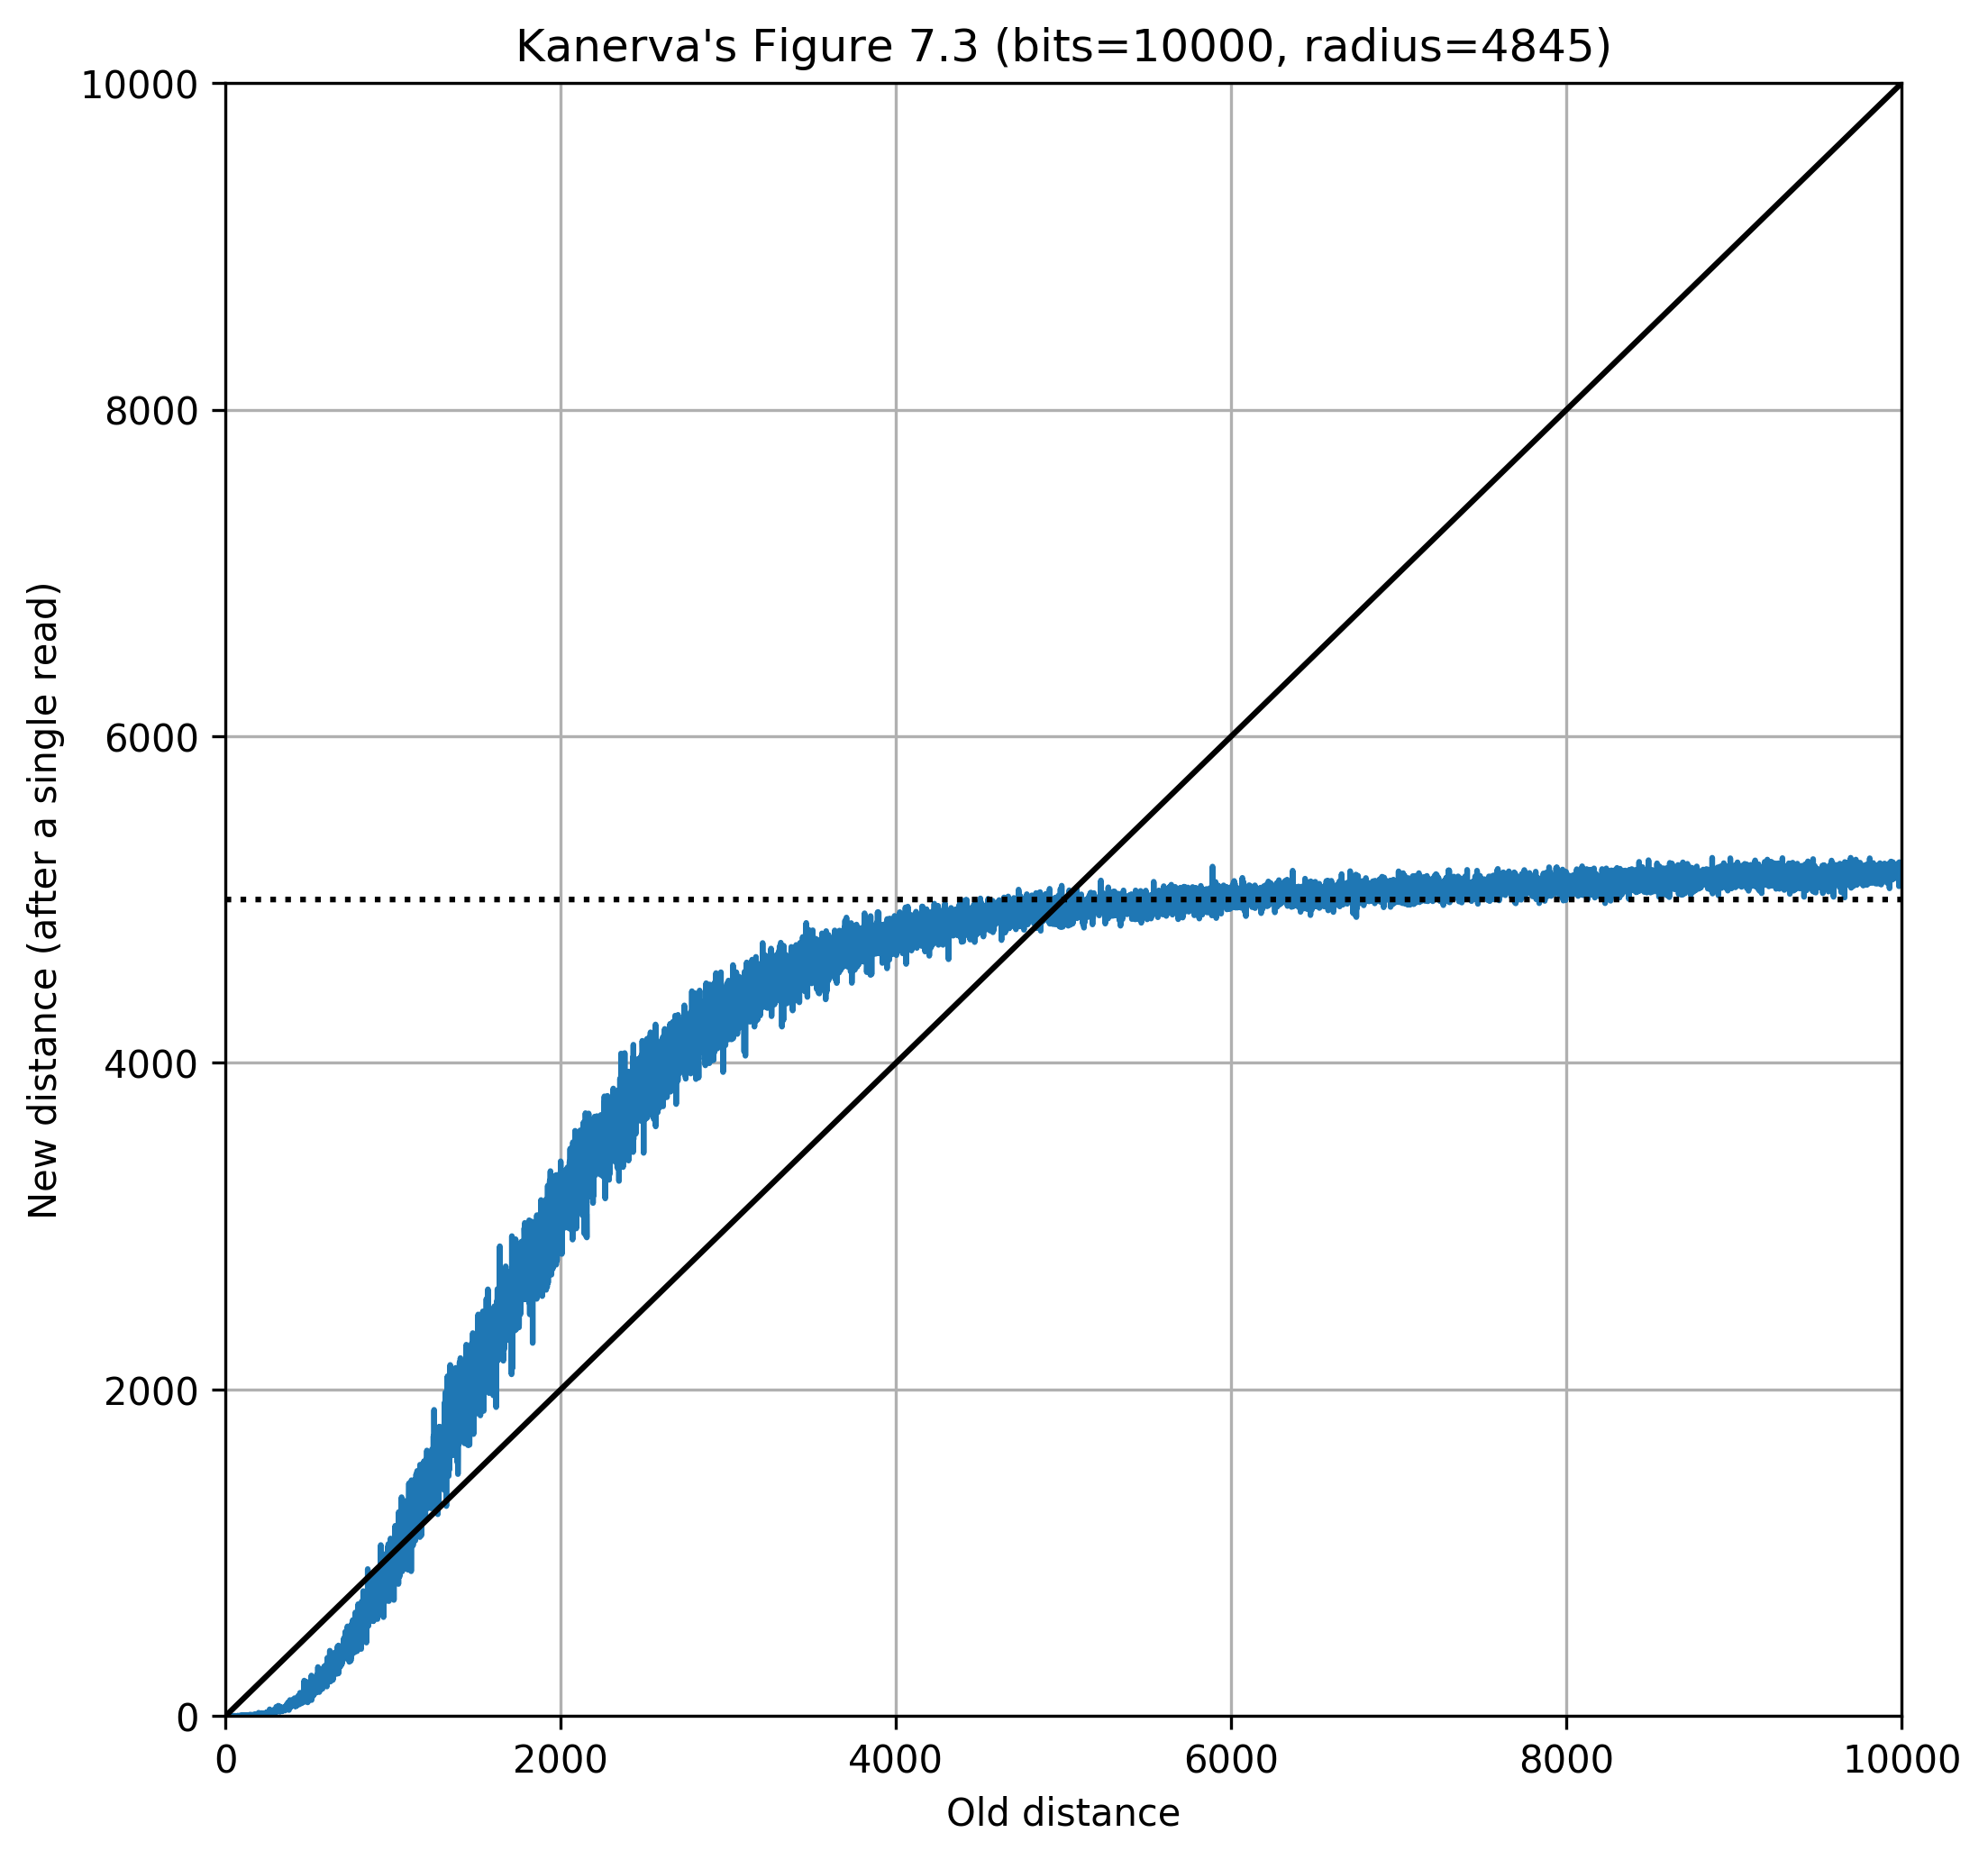
\includegraphics[width=0.75\textwidth]{./images02/sdm-10000bits-10000w-table-7-2.png}

  \caption{The same setup as in Figure \ref{fig:sdm-10000w-table-7-2}, but for $n=10,000$. It shows that the interference has almost gone away when $n$ is sufficiently large.}
  \label{fig:sdm-10kbits-figure-7-3}
\end{figure}

So far we have looked only at a single pair of bitstrings, the probability of a single bitmatch between bitstrings within the access radius distance.  Now let us consider the number of activated hard locations exhibiting this bitmatch.

Let $h$ be the number of activated hard locations. As the probability of activating a specific hard location is constant, $h \sim \text{Binomial}(H, p_1)$. Thus, $\mathbf{E}[h] = \mu_h = Hp_1$ and $\mathbf{V}[h] = \sigma^2_h = Hp_1(1-p_1)$, where $p_1 = 2^{-n} \sum_{k=0}^{r} \binom{n}{k}$.

Let $Z$ be the number of activated hard locations with the same bit as the reading address. Then, $Z = \sum_{i=1}^{h} X_i$, where $X_i \sim \text{Bernoulli}(p)$, where $p = P(x_i = y_i | d(x, y) \le r)$.

\begin{theorem}
Given a reading address $x$ and a dimension $i$, the number of activated hard-locations with bitmatches at $i$ follows a normal distribution with $\mathbf{E}[Z] = \mu_Z = p \mu_h$ and $\mathbf{V}[Z] = \sigma_Z^2 = p(1-p) \mu_h + p^2 \sigma^2_h$.
\label{T2}
\end{theorem}

\begin{proof}
As $P(973 < h < 1170) = 0.997$, by the central limit theorem, $Z$ may be approximated by a normal distribution.

By the central limit theorem, $Z$ is normally distributed.

Applying the law of total averages and the law of total variance, $\mathbf{E}[Z] = \mathbf{E}[\mathbf{E}[Z | h]] = \mathbf{E}[ph] = p \mathbf{E}[h] = ph$, and $\mathbf{V}[Z] = \mathbf{E}[\mathbf{V}[Z|h]] + \mathbf{V}[\mathbf{E}[Z|h]] = \mathbf{E}[hp(1-p)] + \mathbf{V}[ph] = p(1-p) \mathbf{E}[h] + p^2 \mathbf{V}[h] = hp(1-p) + p^2 H p_1 (1-p_1)$.

Applying the law of total variance, $\mathbf{V}[Z] = \mathbf{E}[\mathbf{V}[Z|h]] + \mathbf{V}[\mathbf{E}[Z|h]] = \mathbf{E}[hp(1-p)] + \mathbf{V}[ph] = p(1-p) \mathbf{E}[h] + p^2 \mathbf{V}[h] = p(1-p)\mu_h + p^2 \sigma^2_h$.
\end{proof}


See Figure \ref{fig:sdm-same-bit-histogram} for a comparison between the theoretical model and a simulation.

\begin{figure}[h!]
  \centering
  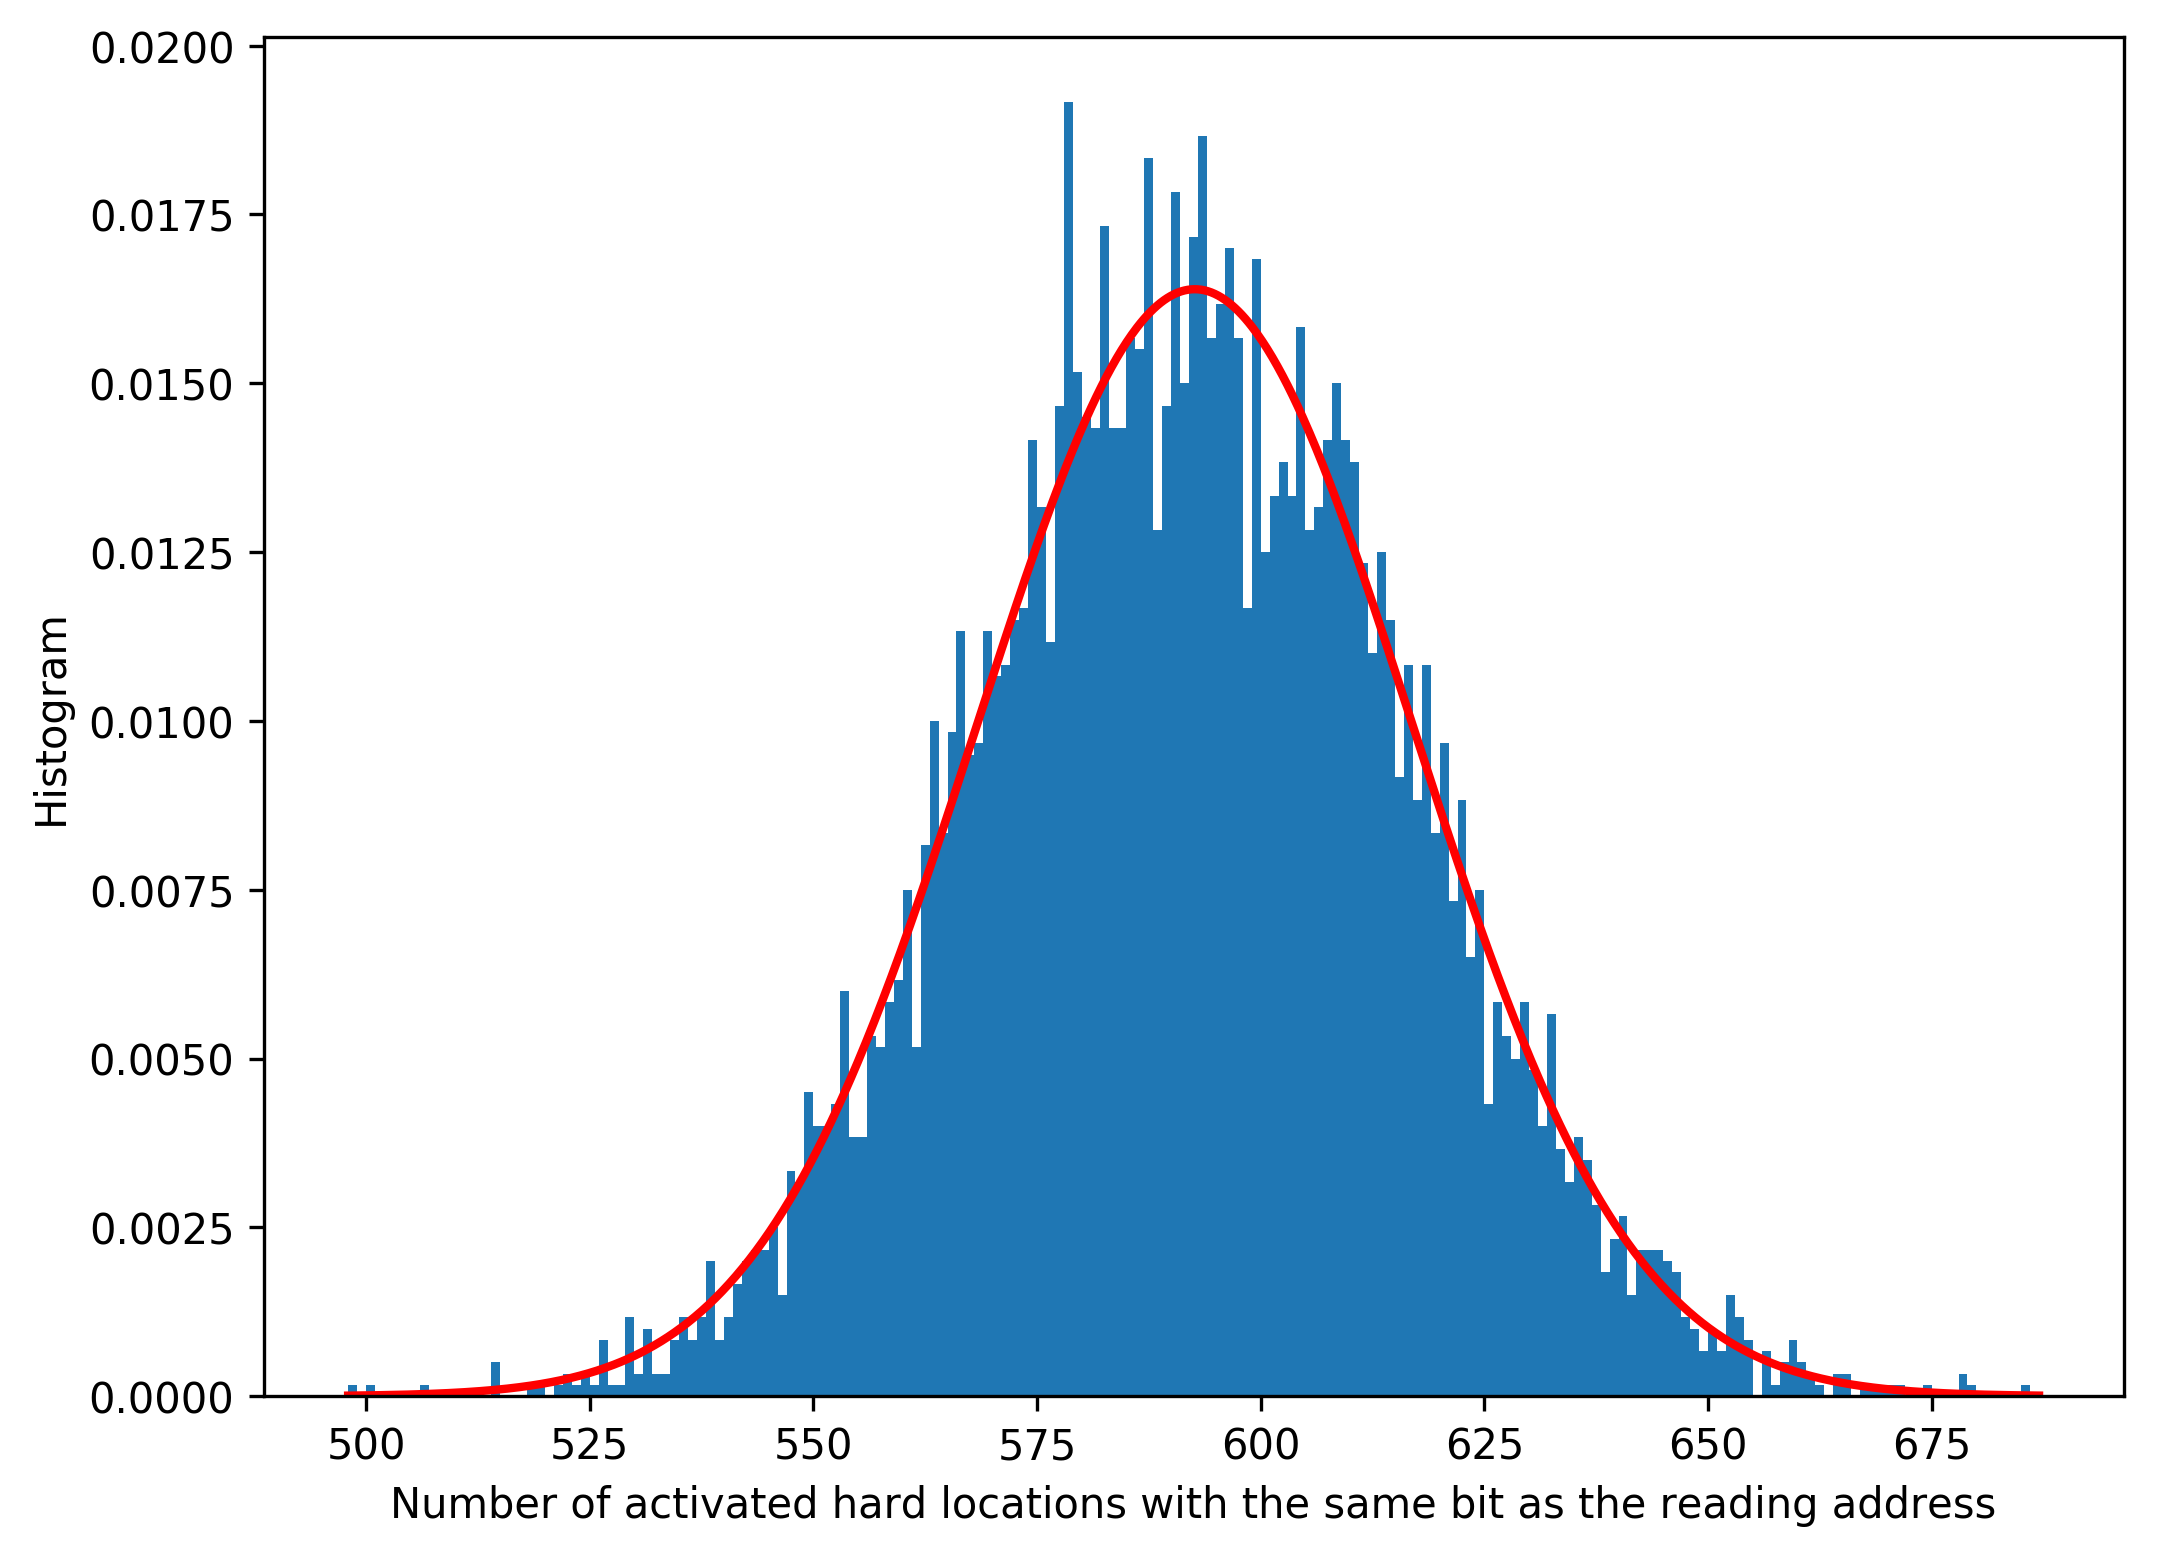
\includegraphics[width=0.75\textwidth]{./images02/autocorrelation/same-bit-histogram.png}

  \caption{Given an address $x$ and a dimension $i$, how many hard locations with bitmatches in $i$ are activated by reading at $x$?  The histogram was obtained through numerical simulation. The red curve is the theoretical normal distribution found in Theorem \ref{T2}.}
  \label{fig:sdm-same-bit-histogram}
\end{figure}

\section{Counter bias}

The previous theorems show that there is bias in the counters. Let us analyze the $i$th counter of a hard location.

Let $s$ be the number of bitstrings written into memory (in our case, $s=10,000$) and $\text{addr}_i$ be the $i$th bit of the hard location's address.

Let $\theta$ be the average number of bitstrings written in each hard location. As there are $s$ bitstrings written into the memory, and the probability of activating a specific hard location is constant, $\theta \sim \text{Binomial}(s, p_1)$. Thus, $\mathbf{E}[\theta] = \mu_\theta = s p_1$ and $\mathbf{V}[\theta] = \sigma^2_\theta = s p_1 (1 - p_1)$.

Let $Y_i$ be the number of bitmatches in the $i$ of a hard location's address after $s$ written bitstrings. Then, $Y_i = \sum_{k=1}^{\theta} X_k$.

\begin{theorem}
Given the number of written bitstrings $s$, $\mathbf{E}[Y_i] = \mu_Y = p \mu_\theta$ and $\mathbf{V}[Y_i] = \sigma^2_Y = p(1-p) \mu_\theta + p^2 \sigma^2_\theta$.
\end{theorem}
\begin{proof}
Applying the law of total expectation, $\mathbf{E}[Y] = \mathbf{E}[\mathbf{E}[Y|\theta]] = \mathbf{E}[p \theta] = p \mathbf{E}[\theta] = p \mu_\theta$.

Applying the law of total variance, $\mathbf{V}[Y] = \mathbf{E}[\mathbf{V}[Y|\theta]] + \mathbf{V}[\mathbf{E}[Y|\theta]] = \mathbf{E}[\theta p (1-p)] + \mathbf{V}[p \theta] = p(1-p) \mathbf{E}[\theta] + p^2 \mathbf{V}[\theta] = p(1-p) \mu_\theta + p^2 \sigma^2_\theta$.
\end{proof}

During a write operation, the counters are incremented for every bit 1 and decremented for every bit 0. So, after $s$ writes, there will be $\theta$ bitstrings written in each hard location with $Y_i$ bitmatches and $\theta - Y_i$ non-bitmatches. Thus, $[\text{cnt}_i | \text{addr}_i = 1] = (Y_i) - (\theta - Y_i) = 2Y_i - \theta$ and $[\text{cnt}_i | \text{addr}_i = 0] = \theta - 2Y_i$.

\begin{theorem}
$\mathbf{E}[\text{cnt}_i | \text{addr}_i = 1] = \mu_{\text{cnt}} = (2p-1) \mu_\theta$ and $\mathbf{V}[\text{cnt}_i | \text{addr}_i = 1] = \sigma^2_\text{cnt} = 4p(1-p) \mu_\theta + (2p-1)^2 \sigma^2_\theta$.
\end{theorem}

\begin{proof}

$\mathbf{E}[\text{cnt}_i | \text{addr}_i = 1] = \mathbf{E}[2Y_i - \theta] = \mathbf{E}[2Y_i] - \mathbf{E}[\theta] = 2 \mathbf{E}[Y_i] - \mu_\theta = 2 p \mu_\theta - \mu_\theta = (2p-1) \mu_\theta$.

Applying the law of total variance, $\mathbf{V}[\text{cnt}_i | \text{addr}_i = 1] = \mathbf{V}[2Y_i - \theta] = \mathbf{E}[\mathbf{V}[2Y_i - \theta | \theta]] + \mathbf{V}[\mathbf{E}[2Y_i - \theta | \theta]]$.

Let us solve each part independently. Thus,

$\mathbf{V}[2Y_i - \theta | \theta] = \mathbf{V}[2Y_i | \theta] = 4 \mathbf{V}[Y_i | \theta] = 4 \mathbf{V}[\sum_{k=1}^\theta X_k] = 4 \theta p (1-p)$.

$\mathbf{E}[\mathbf{V}[2Y_i - \theta | \theta]] = \mathbf{E}[4 \theta p (1-p)] = 4p(1-p) \mathbf{E}[\theta] = 4p(1-p) \mu_\theta$.

Finally,

$\mathbf{E}[2Y_i - \theta | \theta] = 2 \mathbf{E}[Y_i | \theta] - \mathbf{E}[\theta | \theta] = 2p \theta - \theta = (2p-1) \theta$.

$\mathbf{V}[\mathbf{E}[2Y_i - \theta | \theta]] = \mathbf{V}[(2p-1) \theta] = (2p-1)^2 \mathbf{V}[\theta] = (2p-1)^2 \sigma^2_\theta$.
\end{proof}

\begin{theorem}
$\mathbf{E}[\text{cnt}_i | \text{addr}_i = 0] = - \mu_{\text{cnt}}$ and $\mathbf{V}[\text{cnt}_i | \text{addr}_i = 1] = \sigma^2_\text{cnt}$.
\end{theorem}
\begin{proof}
Notice that $[\text{cnt}_i | \text{addr}_i = 0] = -[\text{cnt}_i | \text{addr}_i = 1]$. Thus, $\mathbf{E}[\text{cnt}_i | \text{addr}_i = 0] = -\mathbf{E}[\text{cnt}_i | \text{addr}_i = 1]$ and $\mathbf{V}[\text{cnt}_i | \text{addr}_i = 0] = \mathbf{V}[\text{cnt}_i | \text{addr}_i = 1]$.
\end{proof}

In summary,

\begin{align}
\left[ \text{cnt}_i | \text{addr}_i=1 \right] &\sim \mathcal{N}(\mu_\text{cnt}, \sigma^2_\text{cnt})\label{cntaddr1} \\
\left[ \text{cnt}_i | \text{addr}_i=0 \right] &\sim \mathcal{N}(-\mu_\text{cnt}, \sigma^2_\text{cnt})\label{cntaddr0}
\end{align}

In our case, $p=0.5529$, $s=10,000$, and $H=1,000,000$, so $[\text{cnt}_i | \text{addr}_i=1] \sim \mathcal{N}(\mu=1.1341, \sigma^2 = 10.7184)$. For ``random at x'', $p=0.5$, so $\mu = 0$ and $\sigma^2 = 10.7185$. See Figure \ref{fig:sdm-corr-counters}.

\begin{figure}[h!]
  \centering
  \subfloat[$\text{addr}_i=1$]{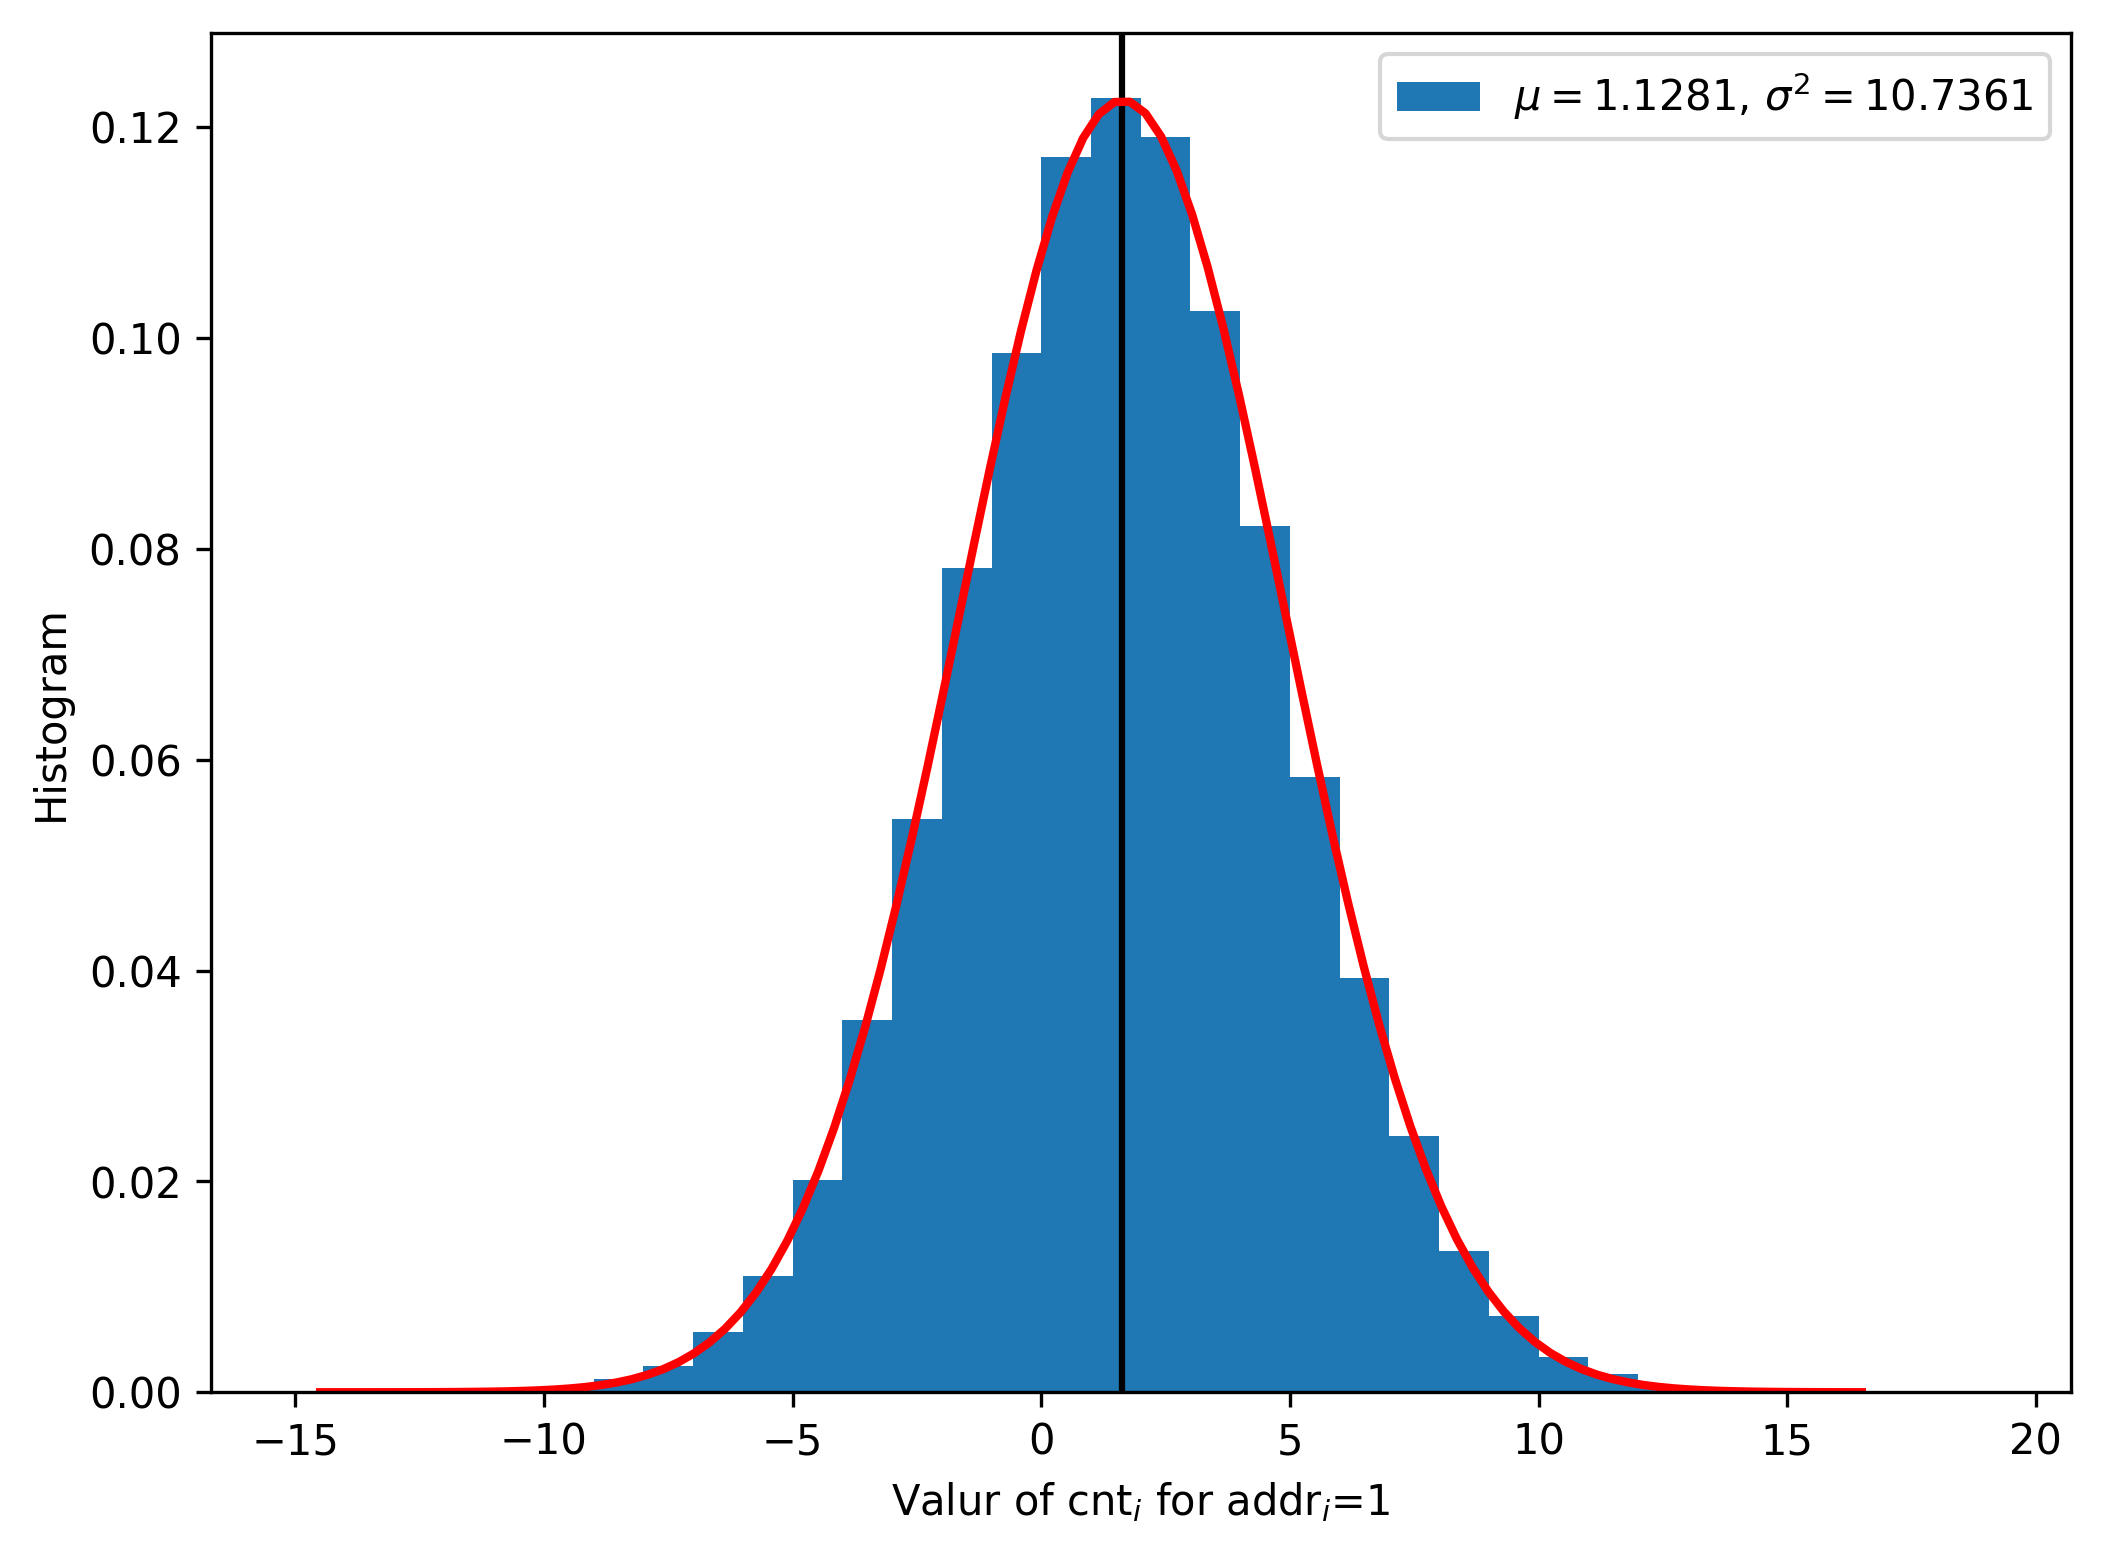
\includegraphics[width=0.5\textwidth]{./images02/autocorrelation/x_at_x_addr1.png}}
  \subfloat[$\text{addr}_i=0$]{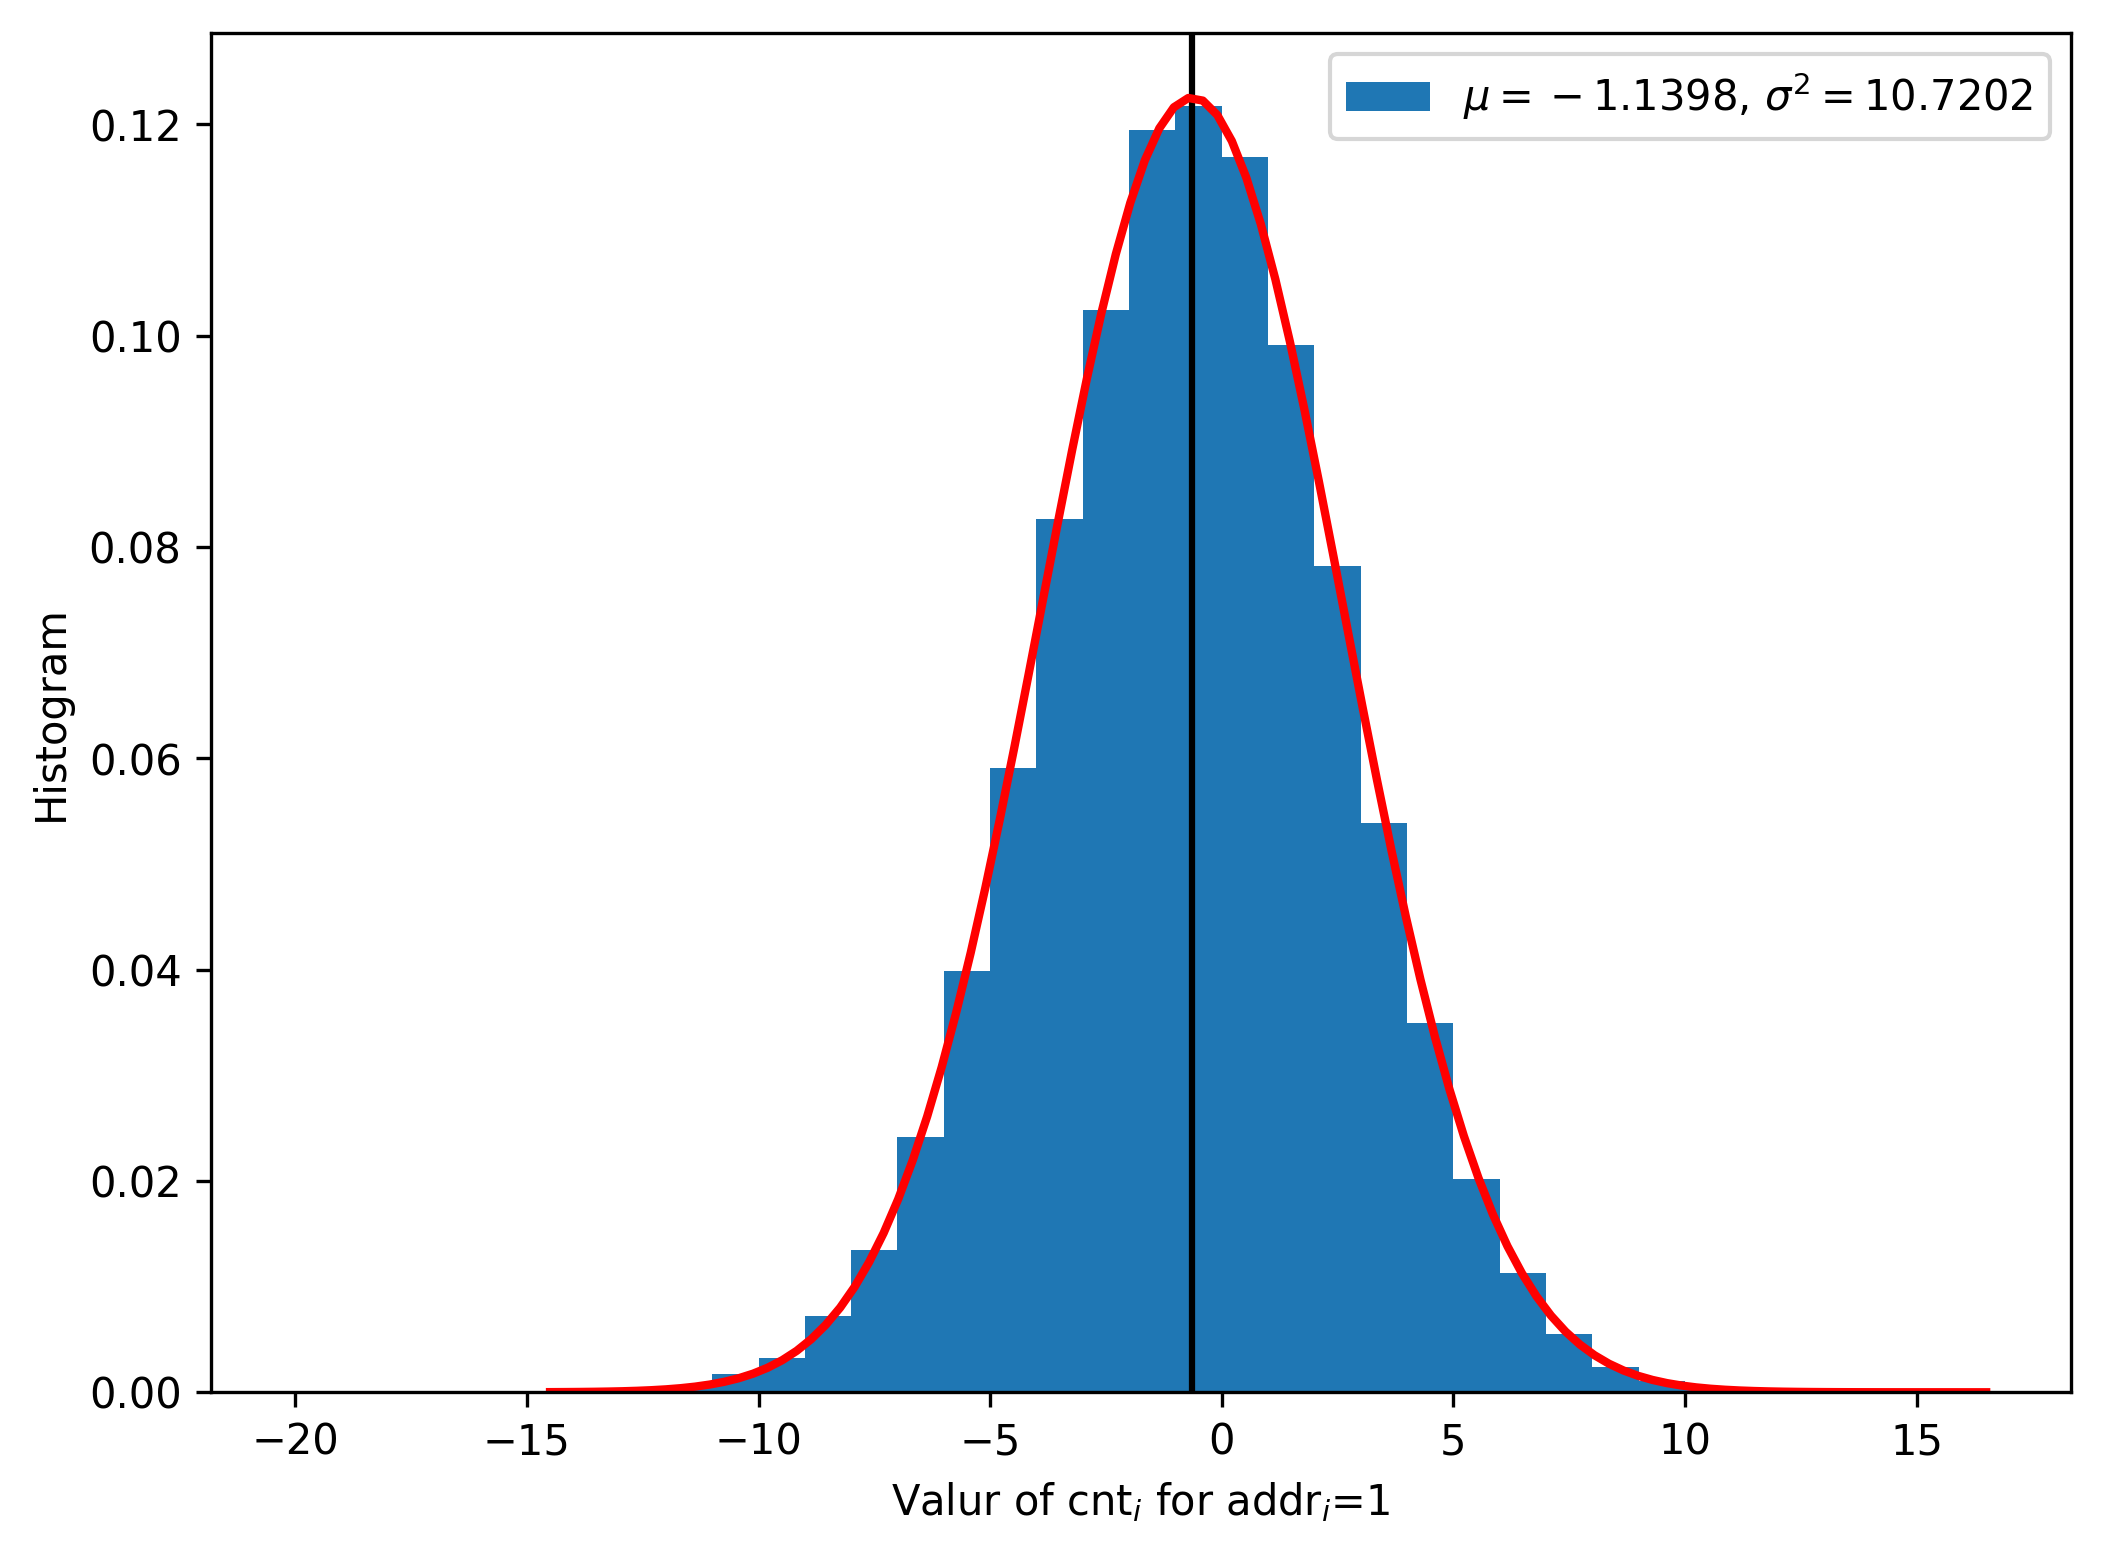
\includegraphics[width=0.5\textwidth]{./images02/autocorrelation/x_at_x_addr0.png}}

  \caption{The value of the counters after $s=10,000$ writes shows the autocorrelation in the counters in autoassociative memories (``x at x''). The histogram was obtained through simulation. The red curve is the theoretical normal distribution found in equations (\ref{cntaddr1}) and (\ref{cntaddr0}).}
  \label{fig:sdm-corr-counters}
\end{figure}


Finally,

\begin{align}
P(\text{cnt}_i > 0 | \text{addr}_i = 1) = P(\text{cnt}_i < 0 | \text{addr}_i = 0) = 1 - \mathcal{N}.\text{cdf}(0)
\end{align}

For ``random written at x'', $p=0.5$ implies $\mu_\text{cnt} = 0$, which implies $P(\text{cnt}_i > 0 | \text{addr}_i = 1) = P(\text{cnt}_i < 0 | \text{addr}_i = 0) = 0.5$, independently of the parameters because they will only affect the variance and the normal distribution is symmetrical around the average.

However, for ``x written at x'', $p=0.5529$ and the probabilities depend on $s$. For $s=10,000$, they are equal to 0.6354. For $s=20,000$, they are equal to 0.6867. For $s=30,000$, they are equal to 0.7232. The more random bitstrings are written into the memory, the more the hard locations point to themselves.

Let $D$ be the number of counters aligned with $\text{addr}_i$. The standard deviation was calculated using the fact that $[D|\theta] \sim \text{Binomial}(1000, q=P(\text{cnt}_i > 0 | \text{addr}_i=1, \theta))$.

Applying the law of total variance, $\mathbf{V}[D] = \mathbf{E}[\mathbf{V}[D|\theta]] + \mathbf{V}[\mathbf{E}[D|\theta]] = \mathbf{E}[1000 q (1-q)] + \mathbf{V}[1000 q] = 1000 \mathbf{E}[q-q^2] + 1000^2 \mathbf{V}[q] = 1000 \mathbf{E}[q](1-\mathbf{E}[q]) + 1000(1000-1)\mathbf{V}[q]$, where $\mathbf{E}[q] = \sum_\theta P(\text{cnt}_i > 0 | \text{addr}_i=1, \theta) P(\theta)$ and $\mathbf{E}[q^2] = \sum_\theta [P(\text{cnt}_i > 0 | \text{addr}_i=1, \theta)]^2 P(\theta)$.

Doing the math, $\mathbf{E}[q] = 0.402922$ and $\mathbf{E}[q^2] = 0.634433$. Thus, $\mathbf{V}[q] = \mathbf{E}[q^2] - (\mathbf{E}[q])^2 = 0.0004166$. Hence, $\mathbf{V}[D] = 648.2041$. See Figure \ref{fig:sdm-corr-prob} and notice that I still have to figure out why the mean is correct, but the standard deviation is not.

\begin{figure}[h!]
  \centering
  \subfloat[``random at x'']{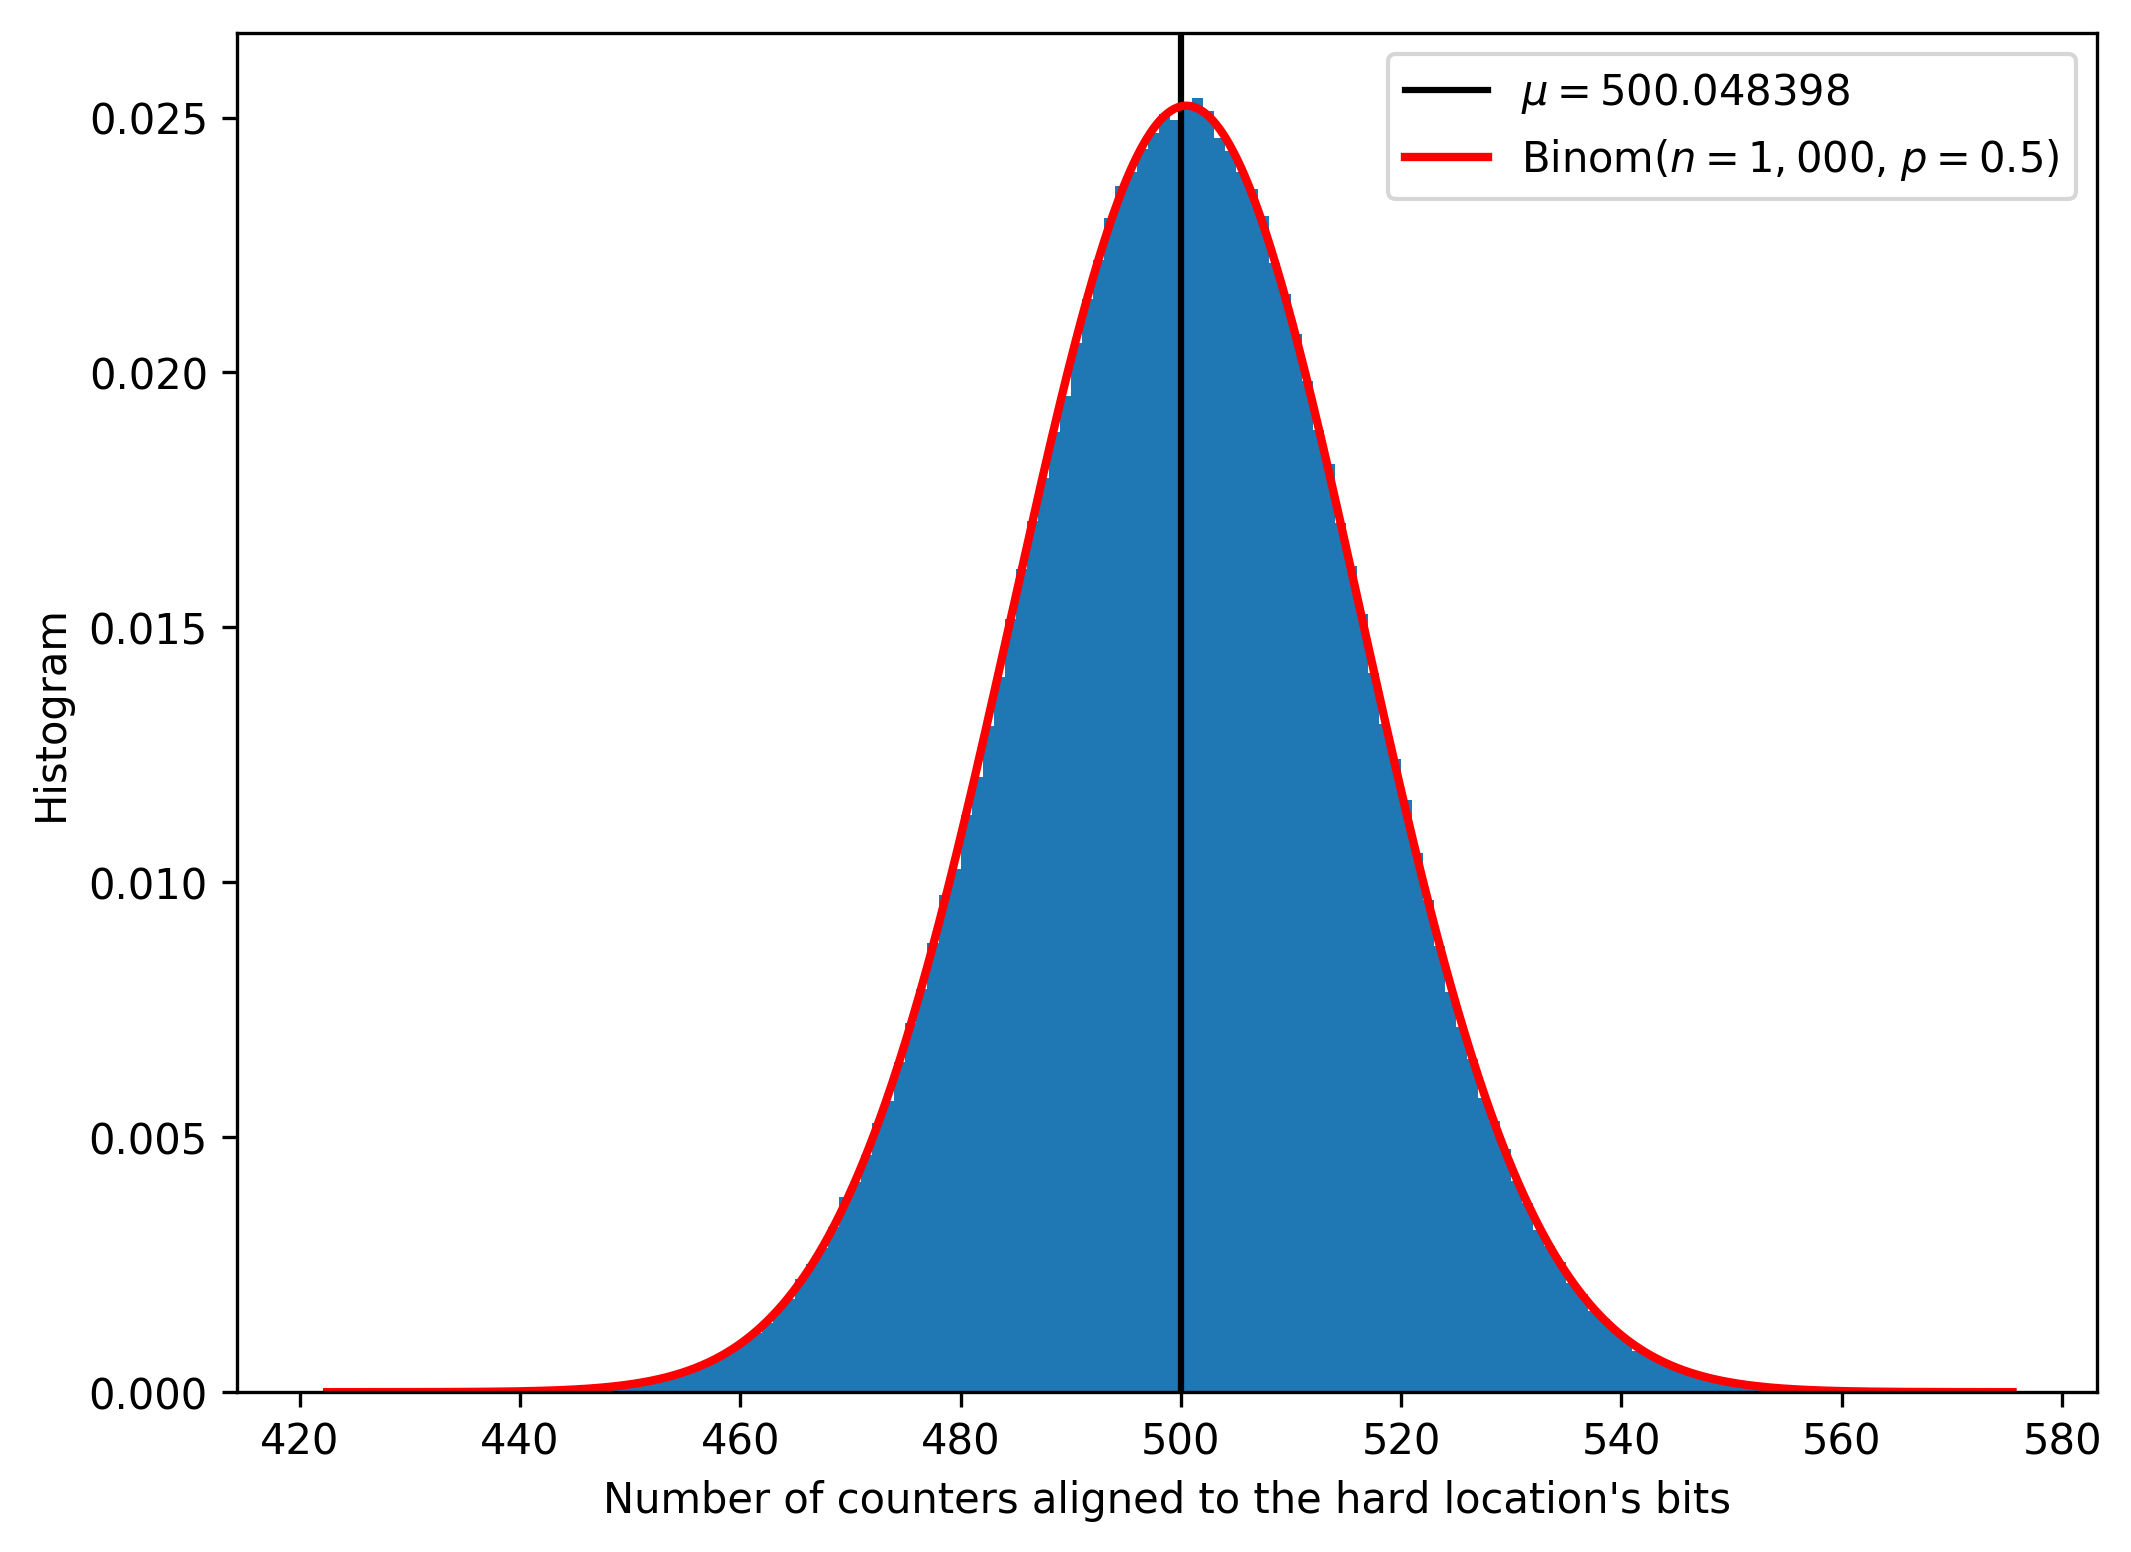
\includegraphics[width=0.5\textwidth]{./images02/autocorrelation/random_at_x_counters.png}}
  \subfloat[``x at x'']{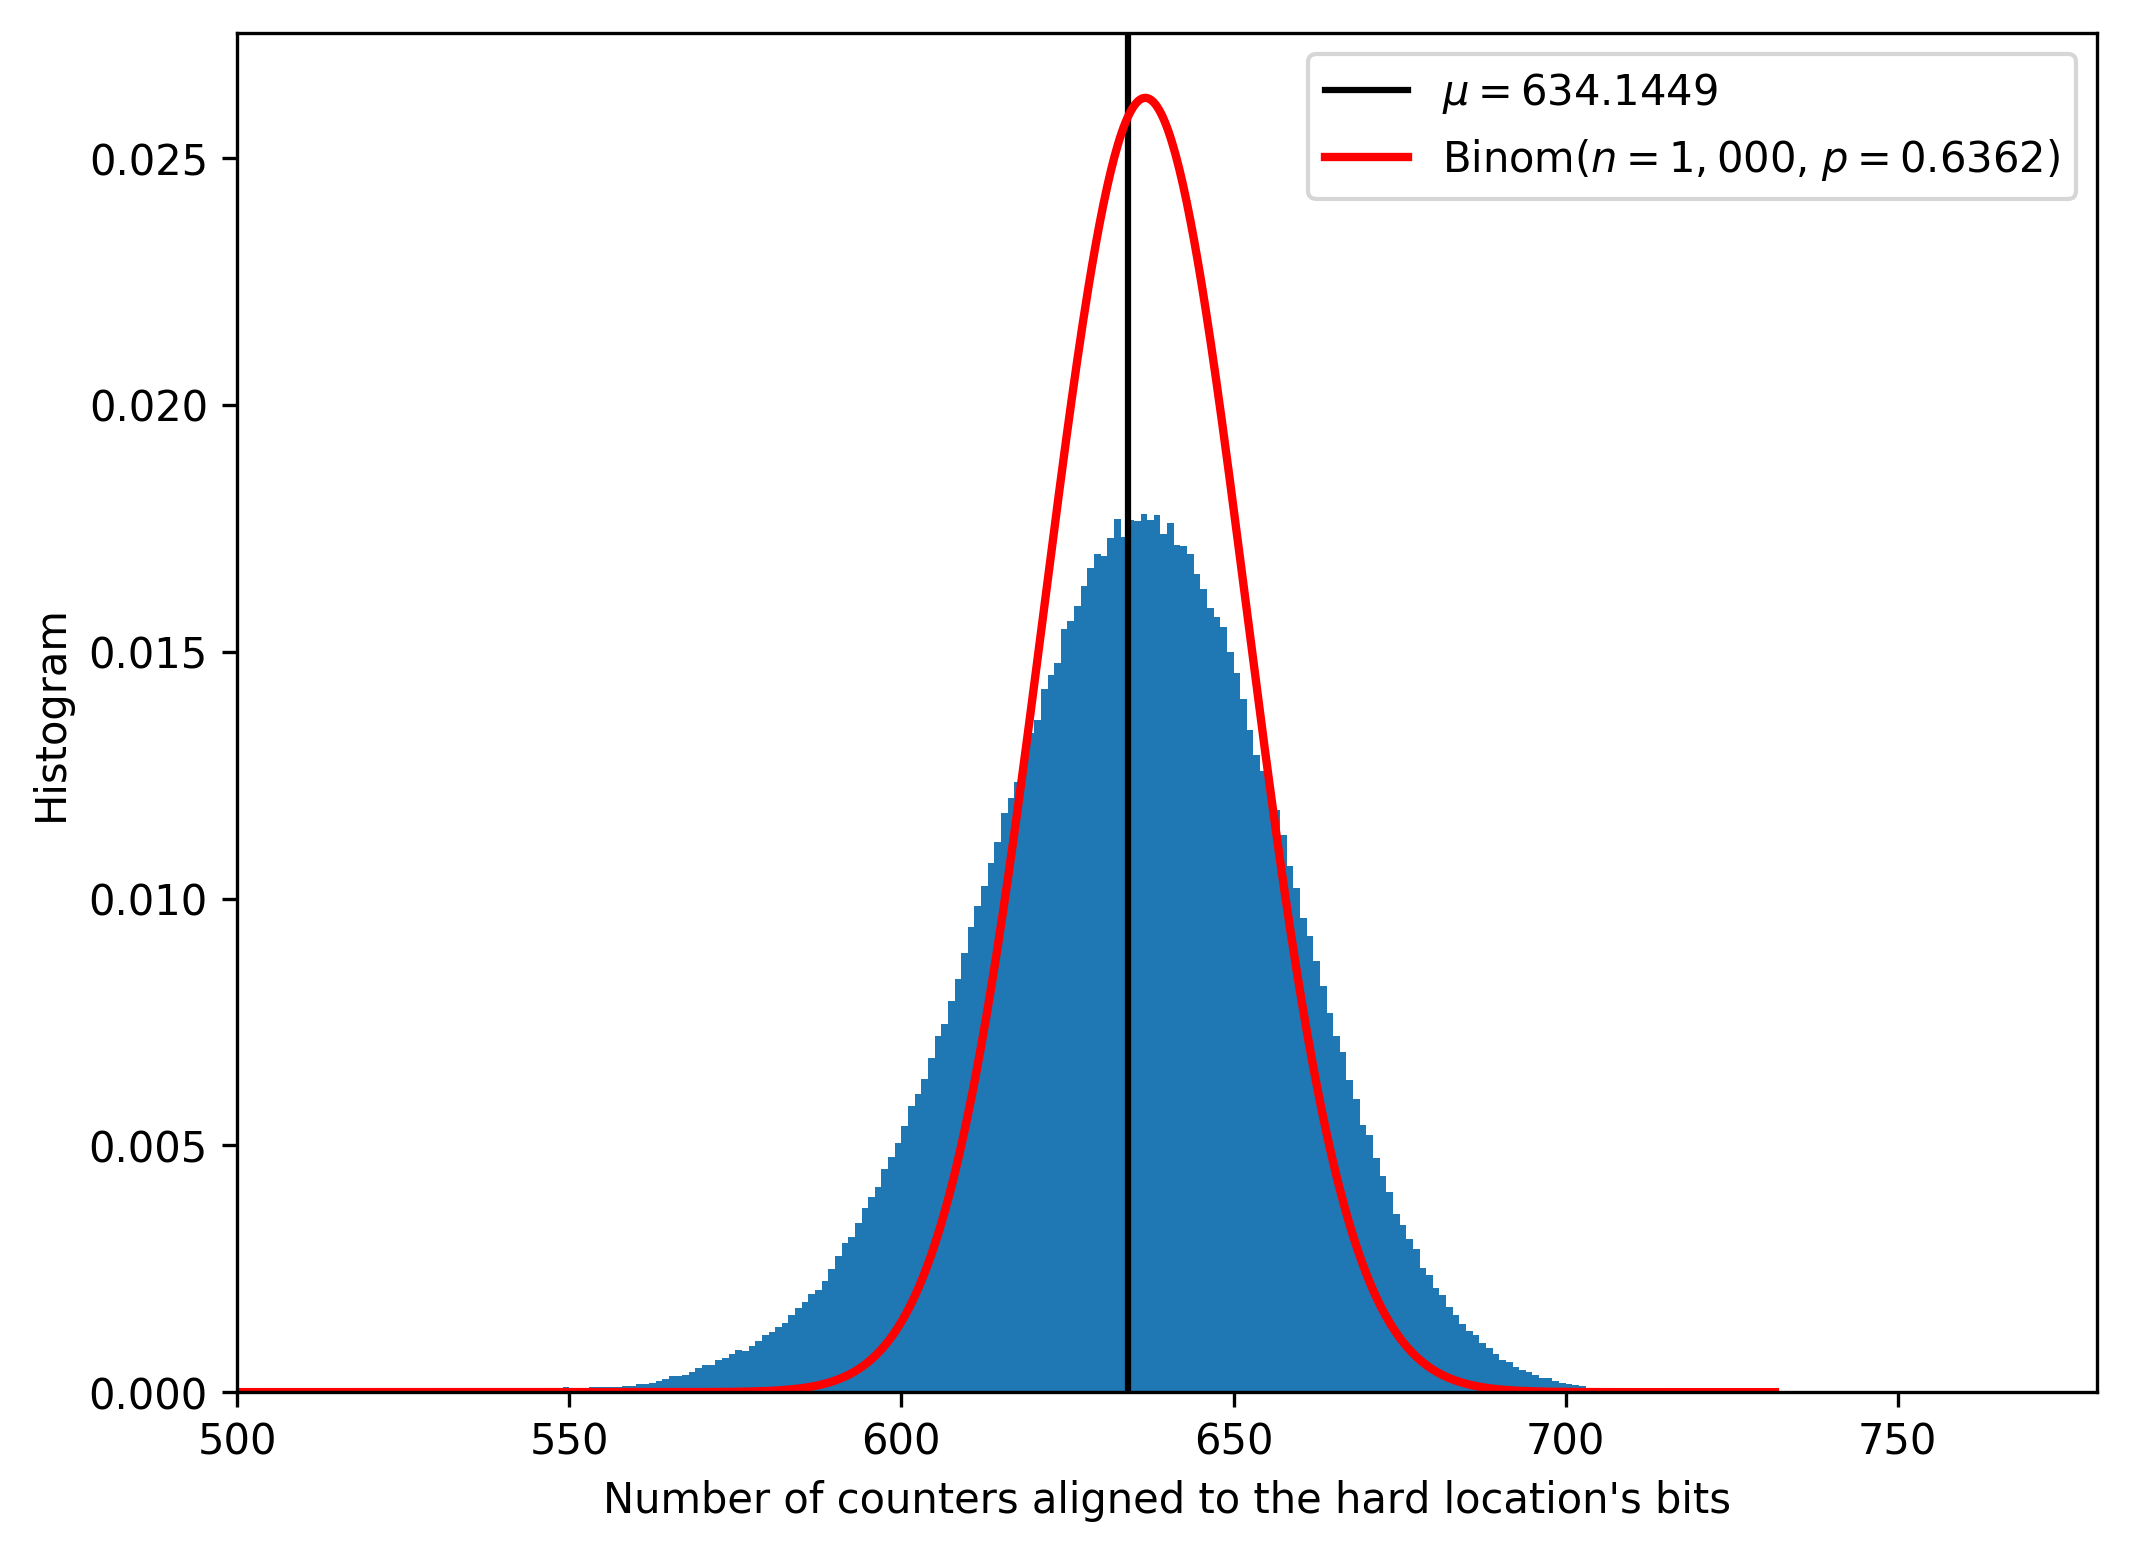
\includegraphics[width=0.5\textwidth]{./images02/autocorrelation/x_at_x_counters.png}}

  \caption{Autocorrelation in the counters in autoassociative memories (``x written at x''). The histogram was obtained through simulation. The red curve is the theoretical distribution.}
  \label{fig:sdm-corr-prob}
\end{figure}



\section{Read bias}

Now that we know the distribution of $\text{cnt}_i | \text{addr}_i$, we may go to the read operation. During the read operation, on average, $h$ hard locations are activated and their counters are summed up. So, for the $i$th bit,

\begin{align}
\text{acc}_i = \sum_{k=1}^{h} \text{cnt}_k
\end{align}

Let $\eta$ be the reading address and $\eta_i$ the $i$th bit of it. Then, let's split the $h$ activated hard locations into two groups: (i) the ones with the same bit as $\eta_i$ with $Z$ hard locations, and (ii) the ones with the opposite bit as $\eta_i$ with $h-Z$ hard locations.

\begin{align}
\left[ \text{acc}_i|\eta_i \right] &= \sum_{k=1}^{Z} \left[ \text{cnt}_k | \text{addr}_k=\eta_i \right] + \sum_{k=1}^{h-Z} \left[ \text{cnt}_k | \text{addr}_k \ne \eta_i \right]
\end{align}

Each sum is a sum of normally distributed random variables, so

\begin{align}
\sum_{k=1}^{Z} \left[ \text{cnt}_k | \text{addr}_k=\eta_1 \right] &\sim \mathcal{N}(\mu = \mu_\text{cnt} \mu_Z, \sigma^2 = \sigma_\text{cnt}^2 \mu_Z + \mu_\text{cnt}^2 \sigma^2_Z) \label{eqn:sdm-eta1-addr1} \\
\sum_{k=1}^{h-Z} \left[ \text{cnt}_k | \text{addr}_k \ne \eta_1 \right] &\sim \mathcal{N}(\mu = -\mu_\text{cnt} (1-p) \mu_h, \sigma^2 = \sigma^2_\text{cnt} (1-p) \mu_h + \mu_\text{cnt}^2 \sigma^2_{h-Z}) \label{eqn:sdm-eta1-addr0}
\end{align}

In our case, $\sum_{k=1}^{Z} \left[ \text{cnt}_k | \text{addr}_k=1 \right] \sim \mathcal{N}(\mu=672.12, \sigma^2=7113.87)$, and $\sum_{k=1}^{Z} \left[ \text{cnt}_k | \text{addr}_k=1 \right] \sim \mathcal{N}(\mu=-543.49, \sigma^2=5752.54)$. See Figure \ref{fig:sdm-read-sums} --- we can notice that the average is correct but the variance is too small.

\begin{figure}[h!]
  \centering
  \subfloat[Equation \ref{eqn:sdm-eta1-addr1}  ($\text{addr}_k=1)$]{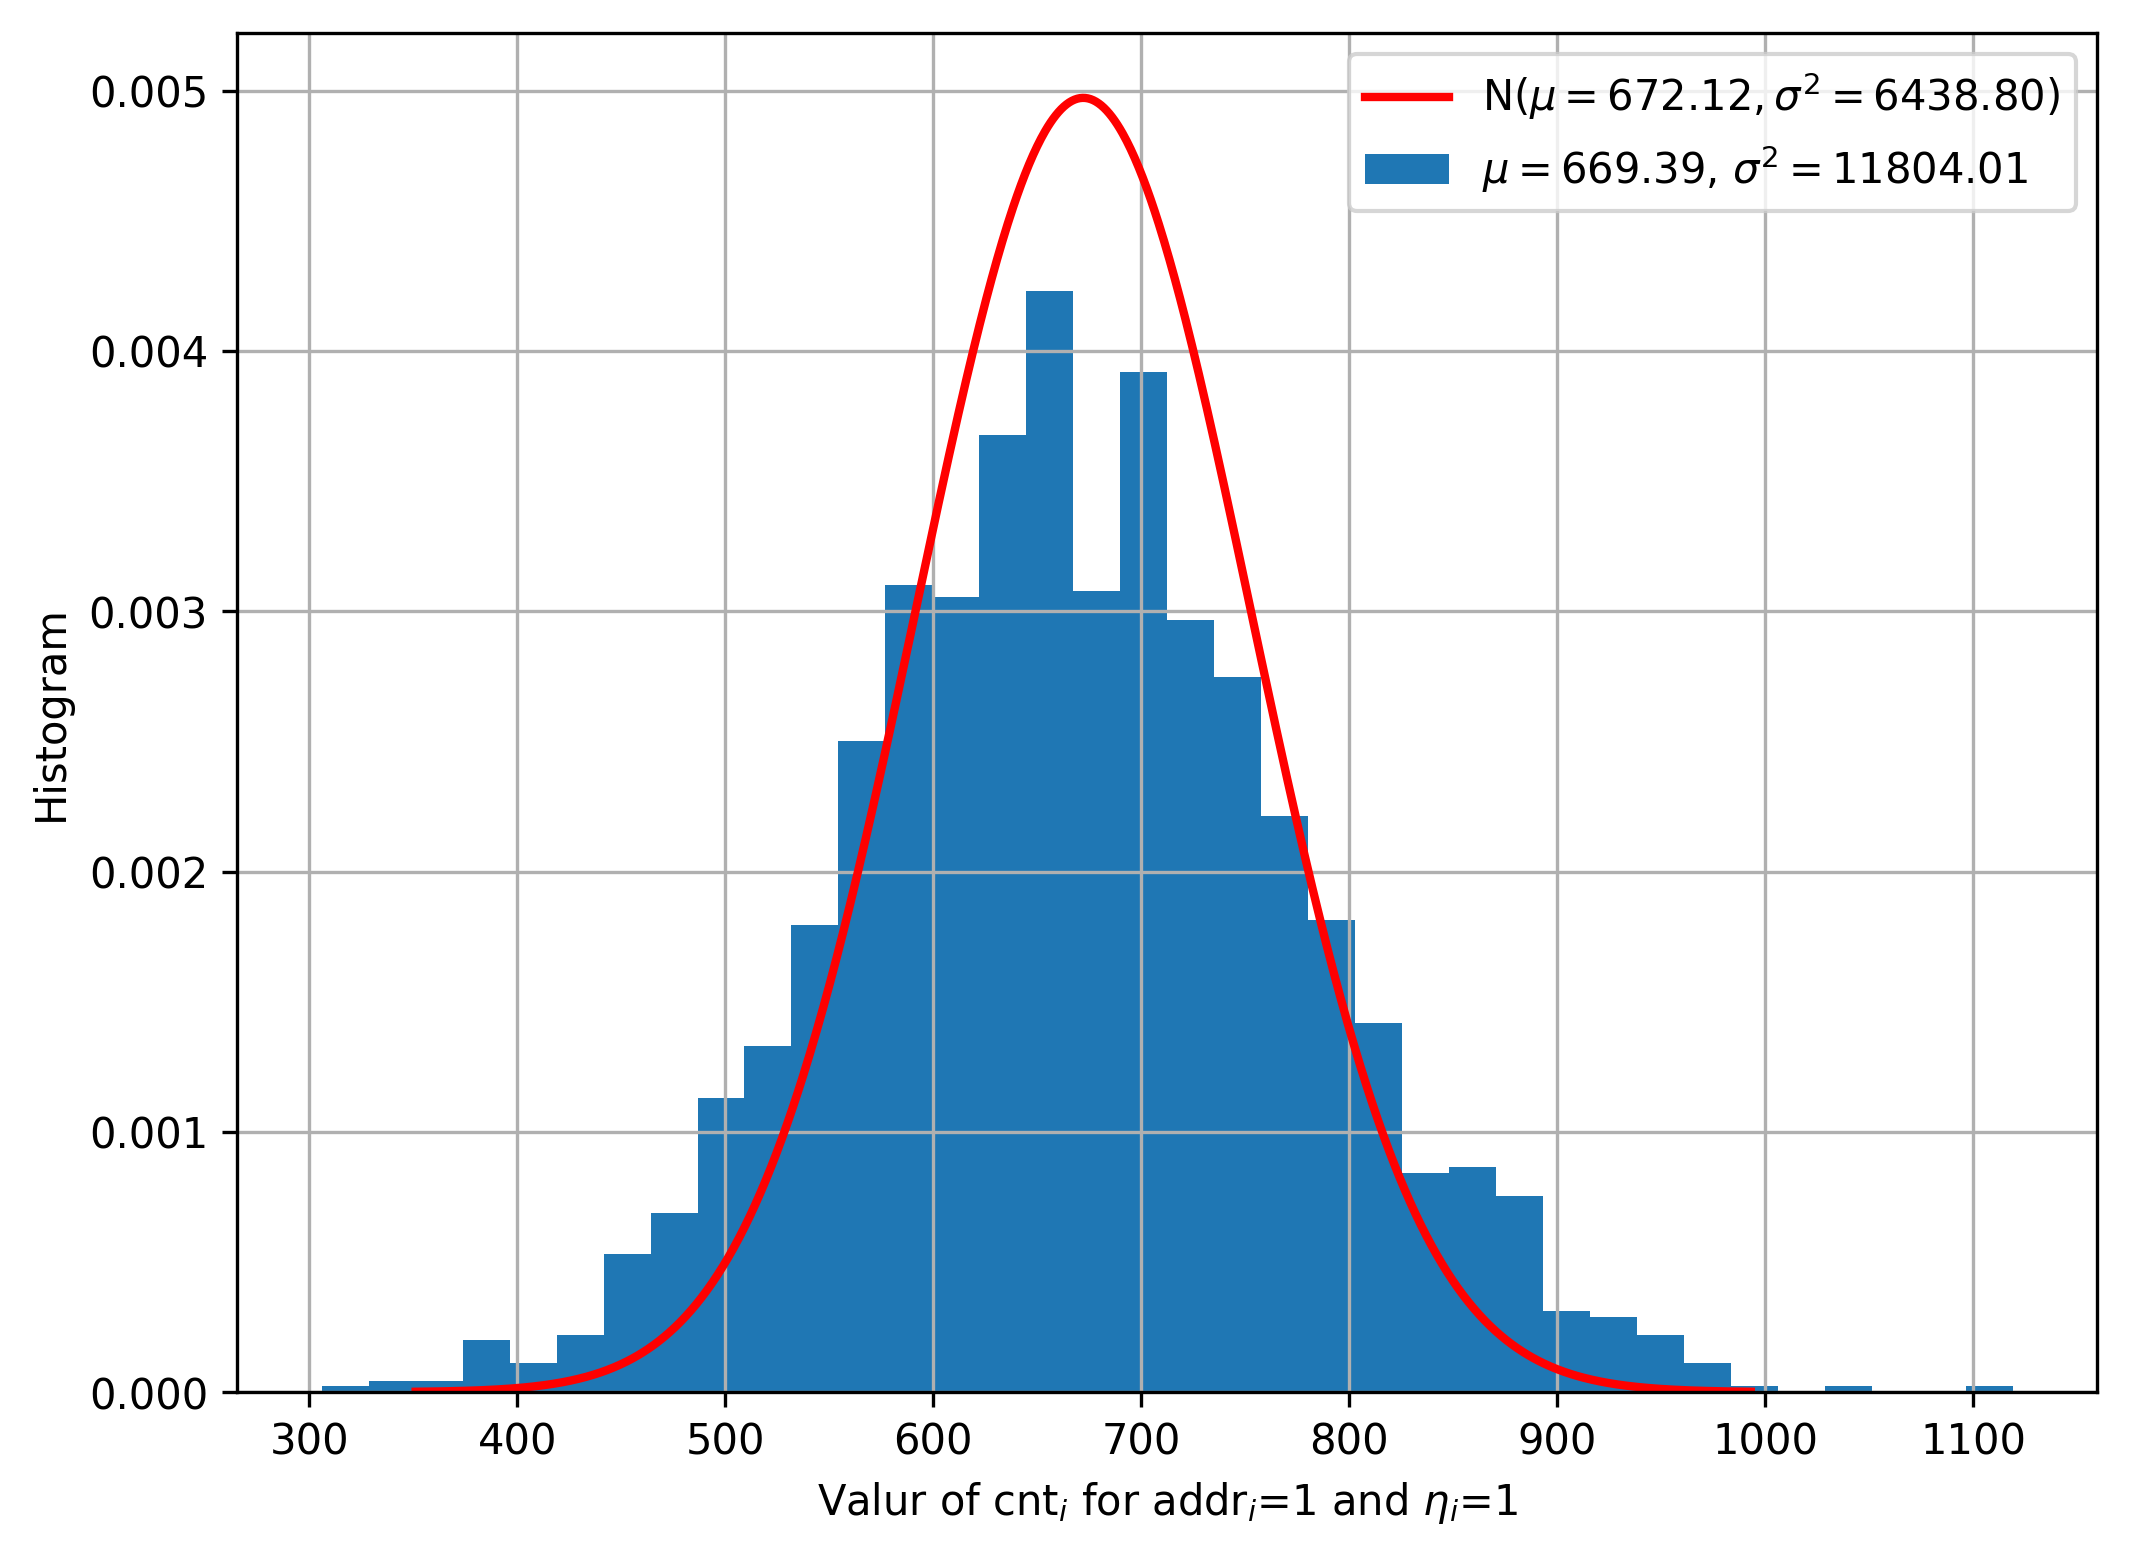
\includegraphics[width=0.5\textwidth]{./images02/autocorrelation/read-counters-eta1_addr1.png}}
  \subfloat[Equation \ref{eqn:sdm-eta1-addr0} ($\text{addr}_k=0$)]{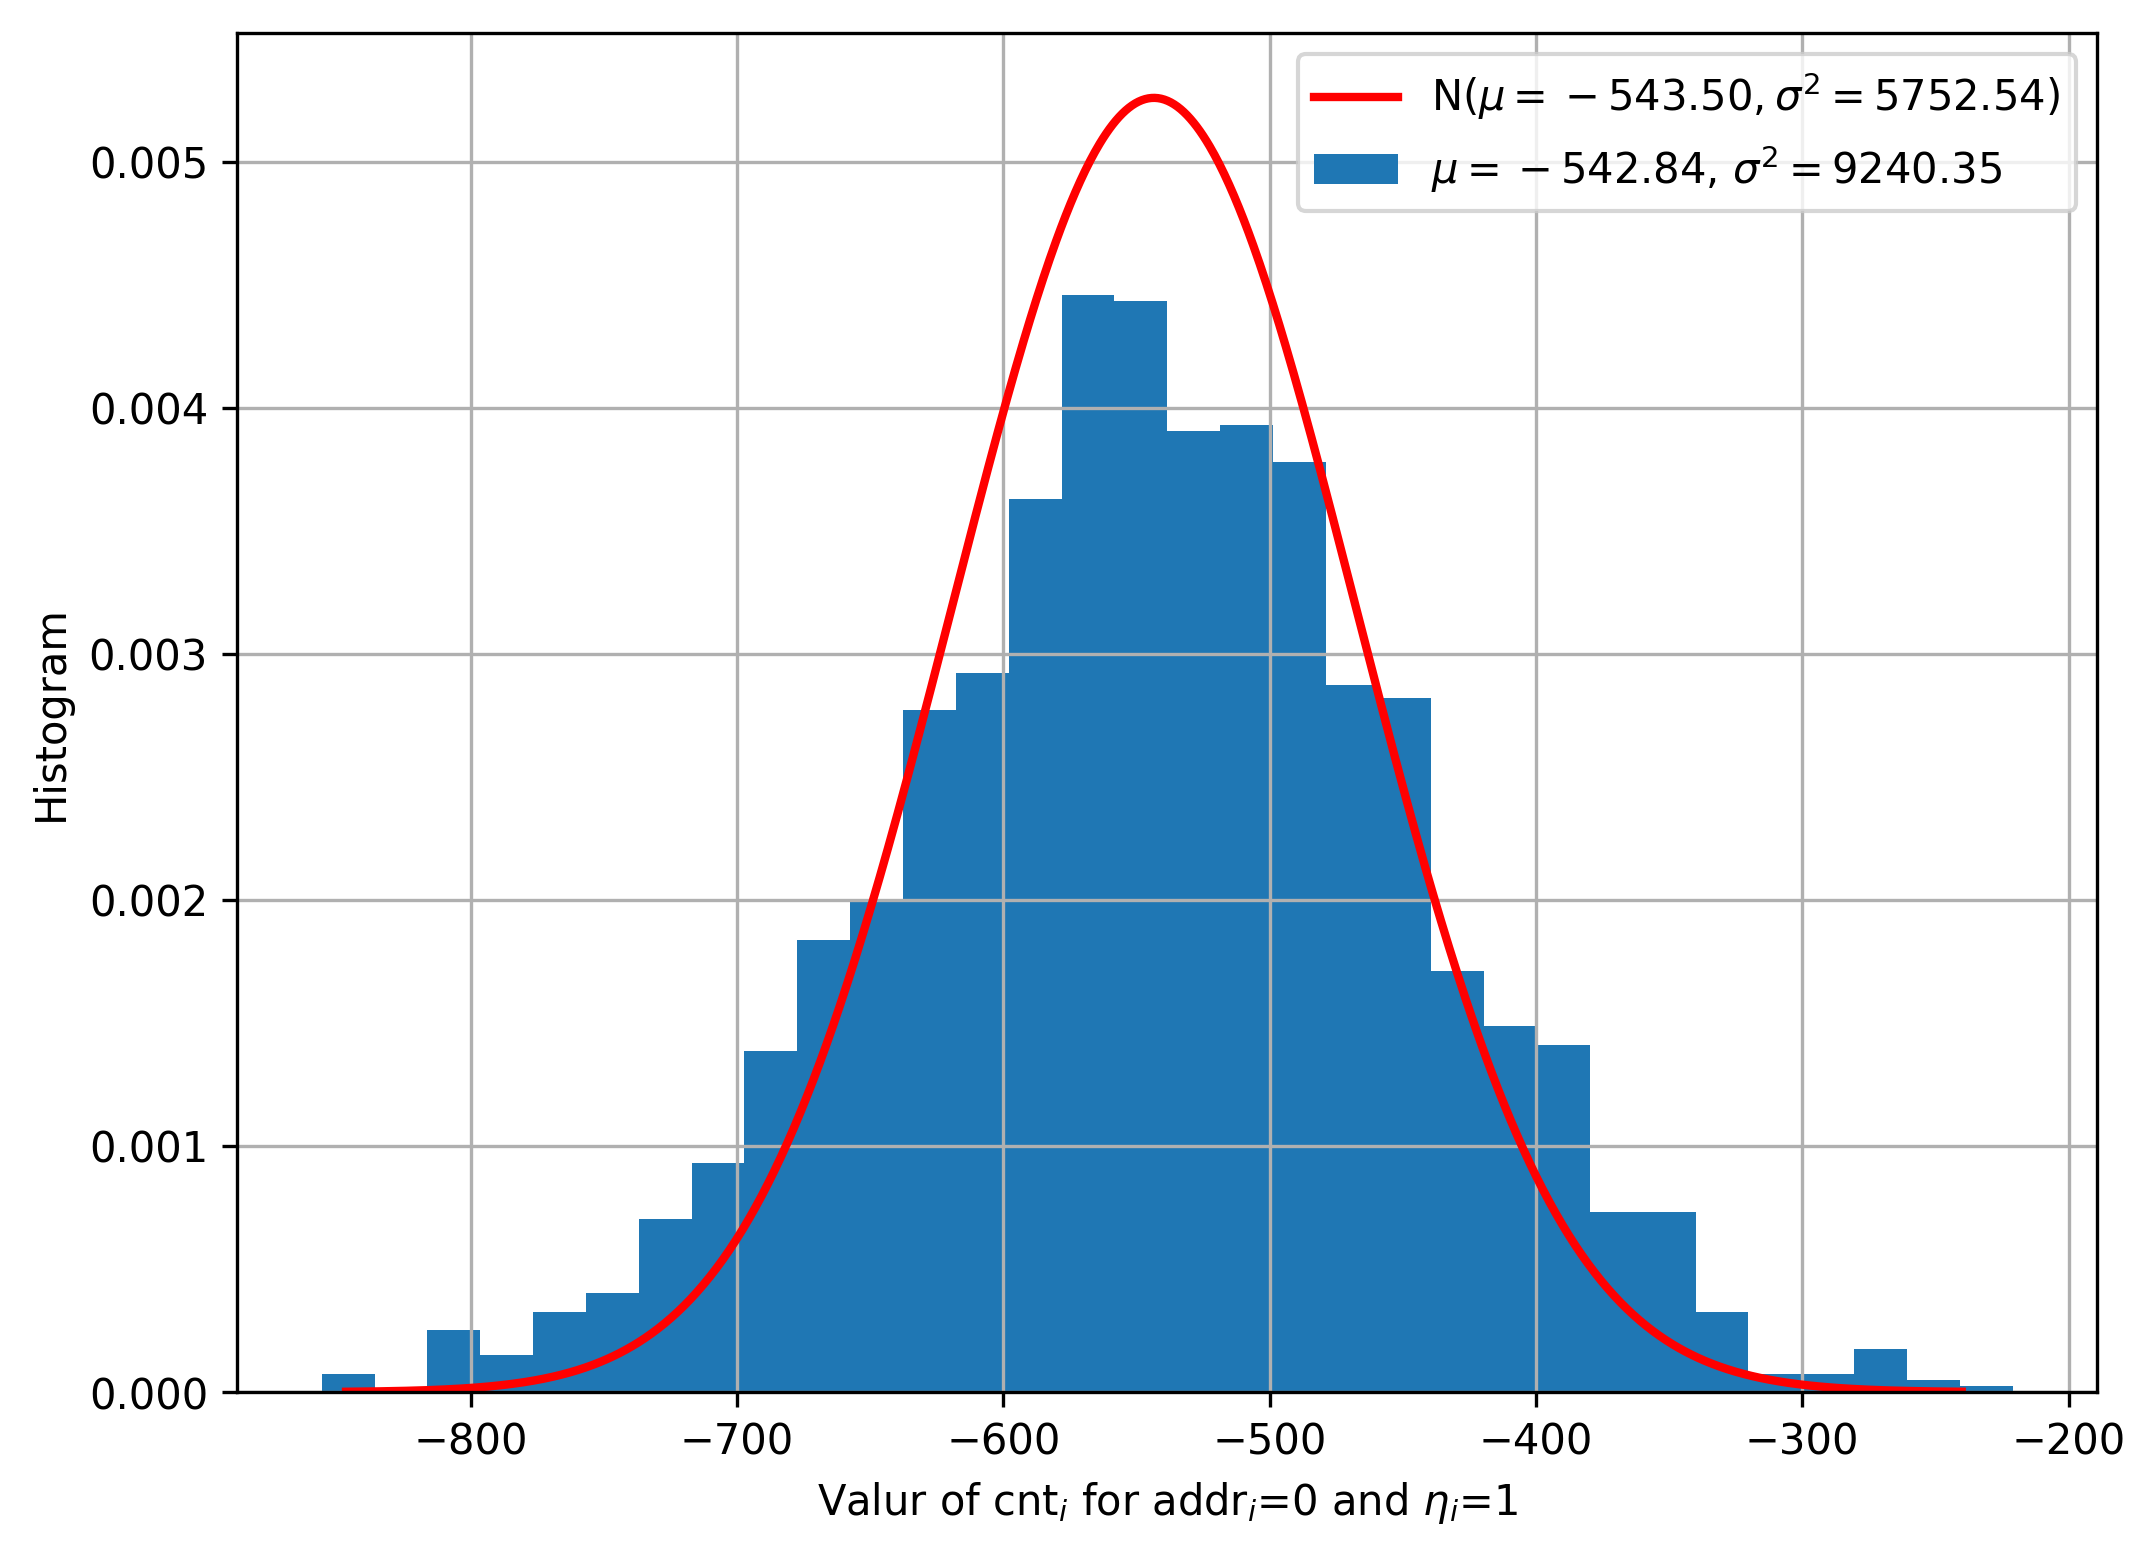
\includegraphics[width=0.5\textwidth]{./images02/autocorrelation/read-counters-eta1_addr0.png}}

  \caption{The histogram was obtained through simulation. The red curve is the theoretical normal distribution.}
  \label{fig:sdm-read-sums}
\end{figure}

Hence,

\begin{align}
\left[ \text{acc}_i|\eta_i=1 \right] &\sim \mathcal{N}(\mu = (2p-1)^2 \mu_\theta \mu_h, \sigma^2 = \sigma_\text{cnt}^2 \mu_h + 2 \mu_\text{cnt}^2 \sigma^2_h) \label{eqn:sdm-eta1} \\
\left[ \text{acc}_i|\eta_i=0 \right] &\sim \mathcal{N}(\mu = -(2p-1)^2 \mu_\theta \mu_h, \sigma^2 = \sigma_\text{cnt}^2 \mu_h + 2 \mu_\text{cnt}^2 \sigma^2_h) \label{eqn:sdm-eta0}
\end{align}

In our case, $\left[ \text{acc}_i|\eta_i=1 \right] \sim \mathcal{N}(\mu = 128.62, \sigma^2 = 12865.69)$, and $\left[ \text{acc}_i|\eta_i=0 \right] \sim \mathcal{N}(\mu = -128.62, \sigma^2 = 12865.69)$. See Figure \ref{fig:sdm-read} --- we can notice that the variance issue from Figure \ref{fig:sdm-read-sums} has propagated to these images.

\begin{figure}[h!]
  \centering
  \subfloat[Equation \ref{eqn:sdm-eta1}  ($\eta_k=1)$]{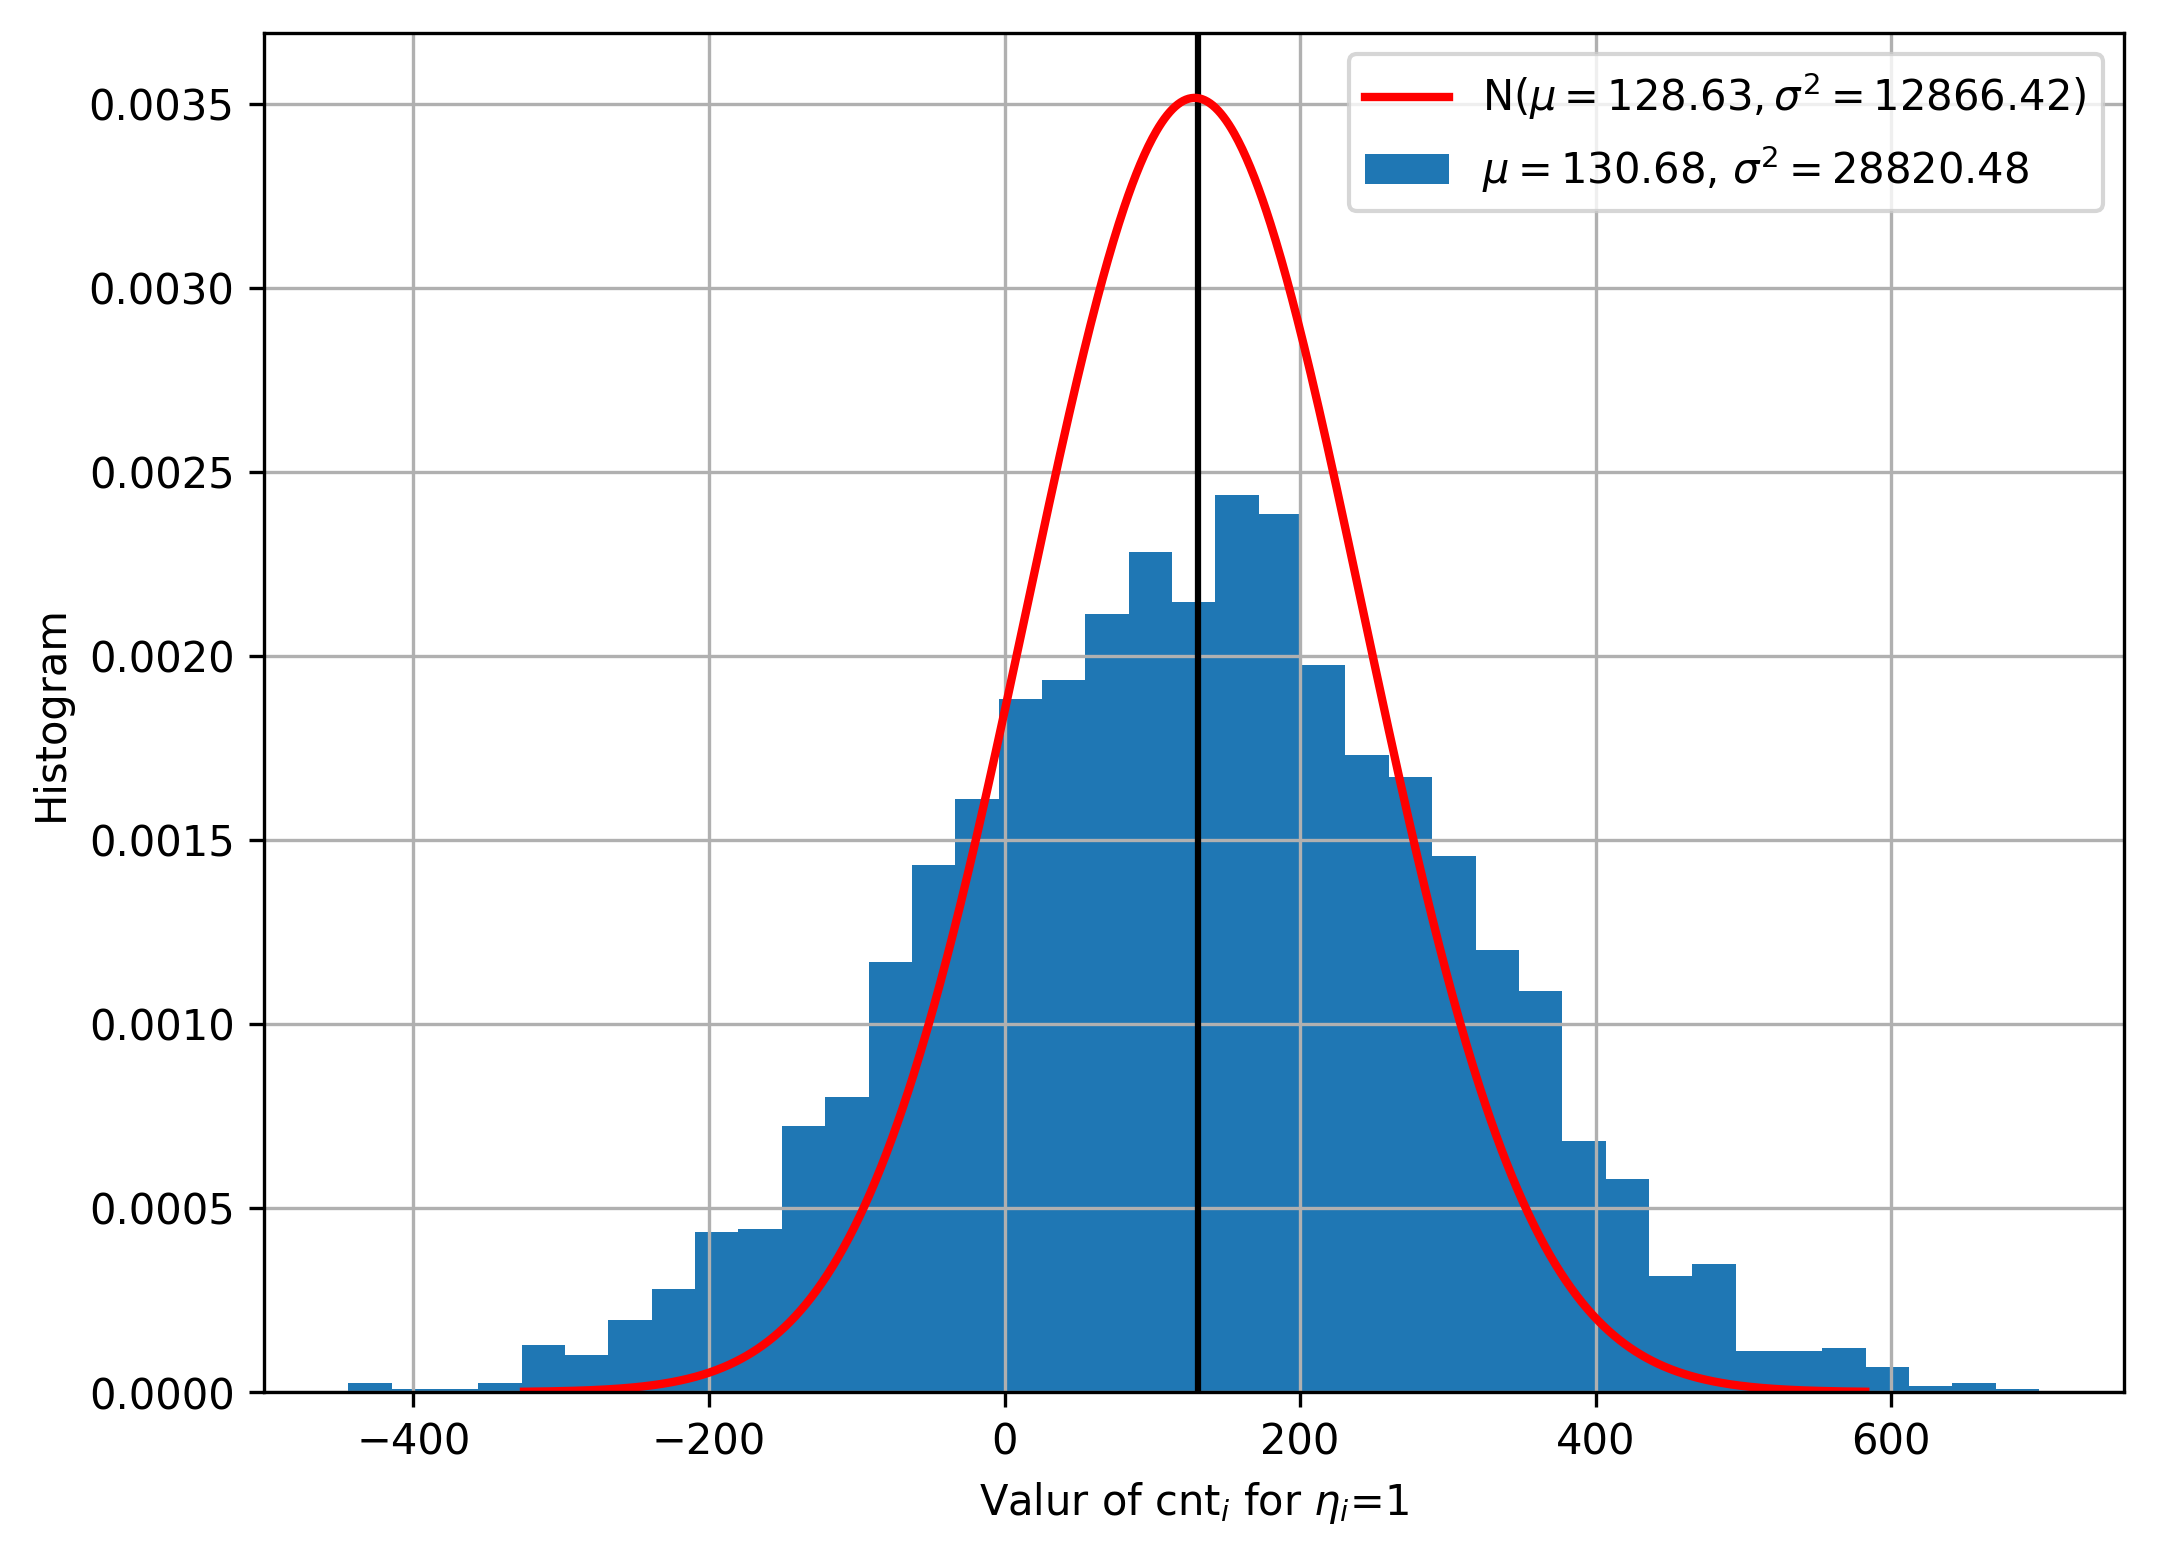
\includegraphics[width=0.5\textwidth]{./images02/autocorrelation/read-counters-eta1.png}}
  \subfloat[Equation \ref{eqn:sdm-eta0} ($\eta_k=0$)]{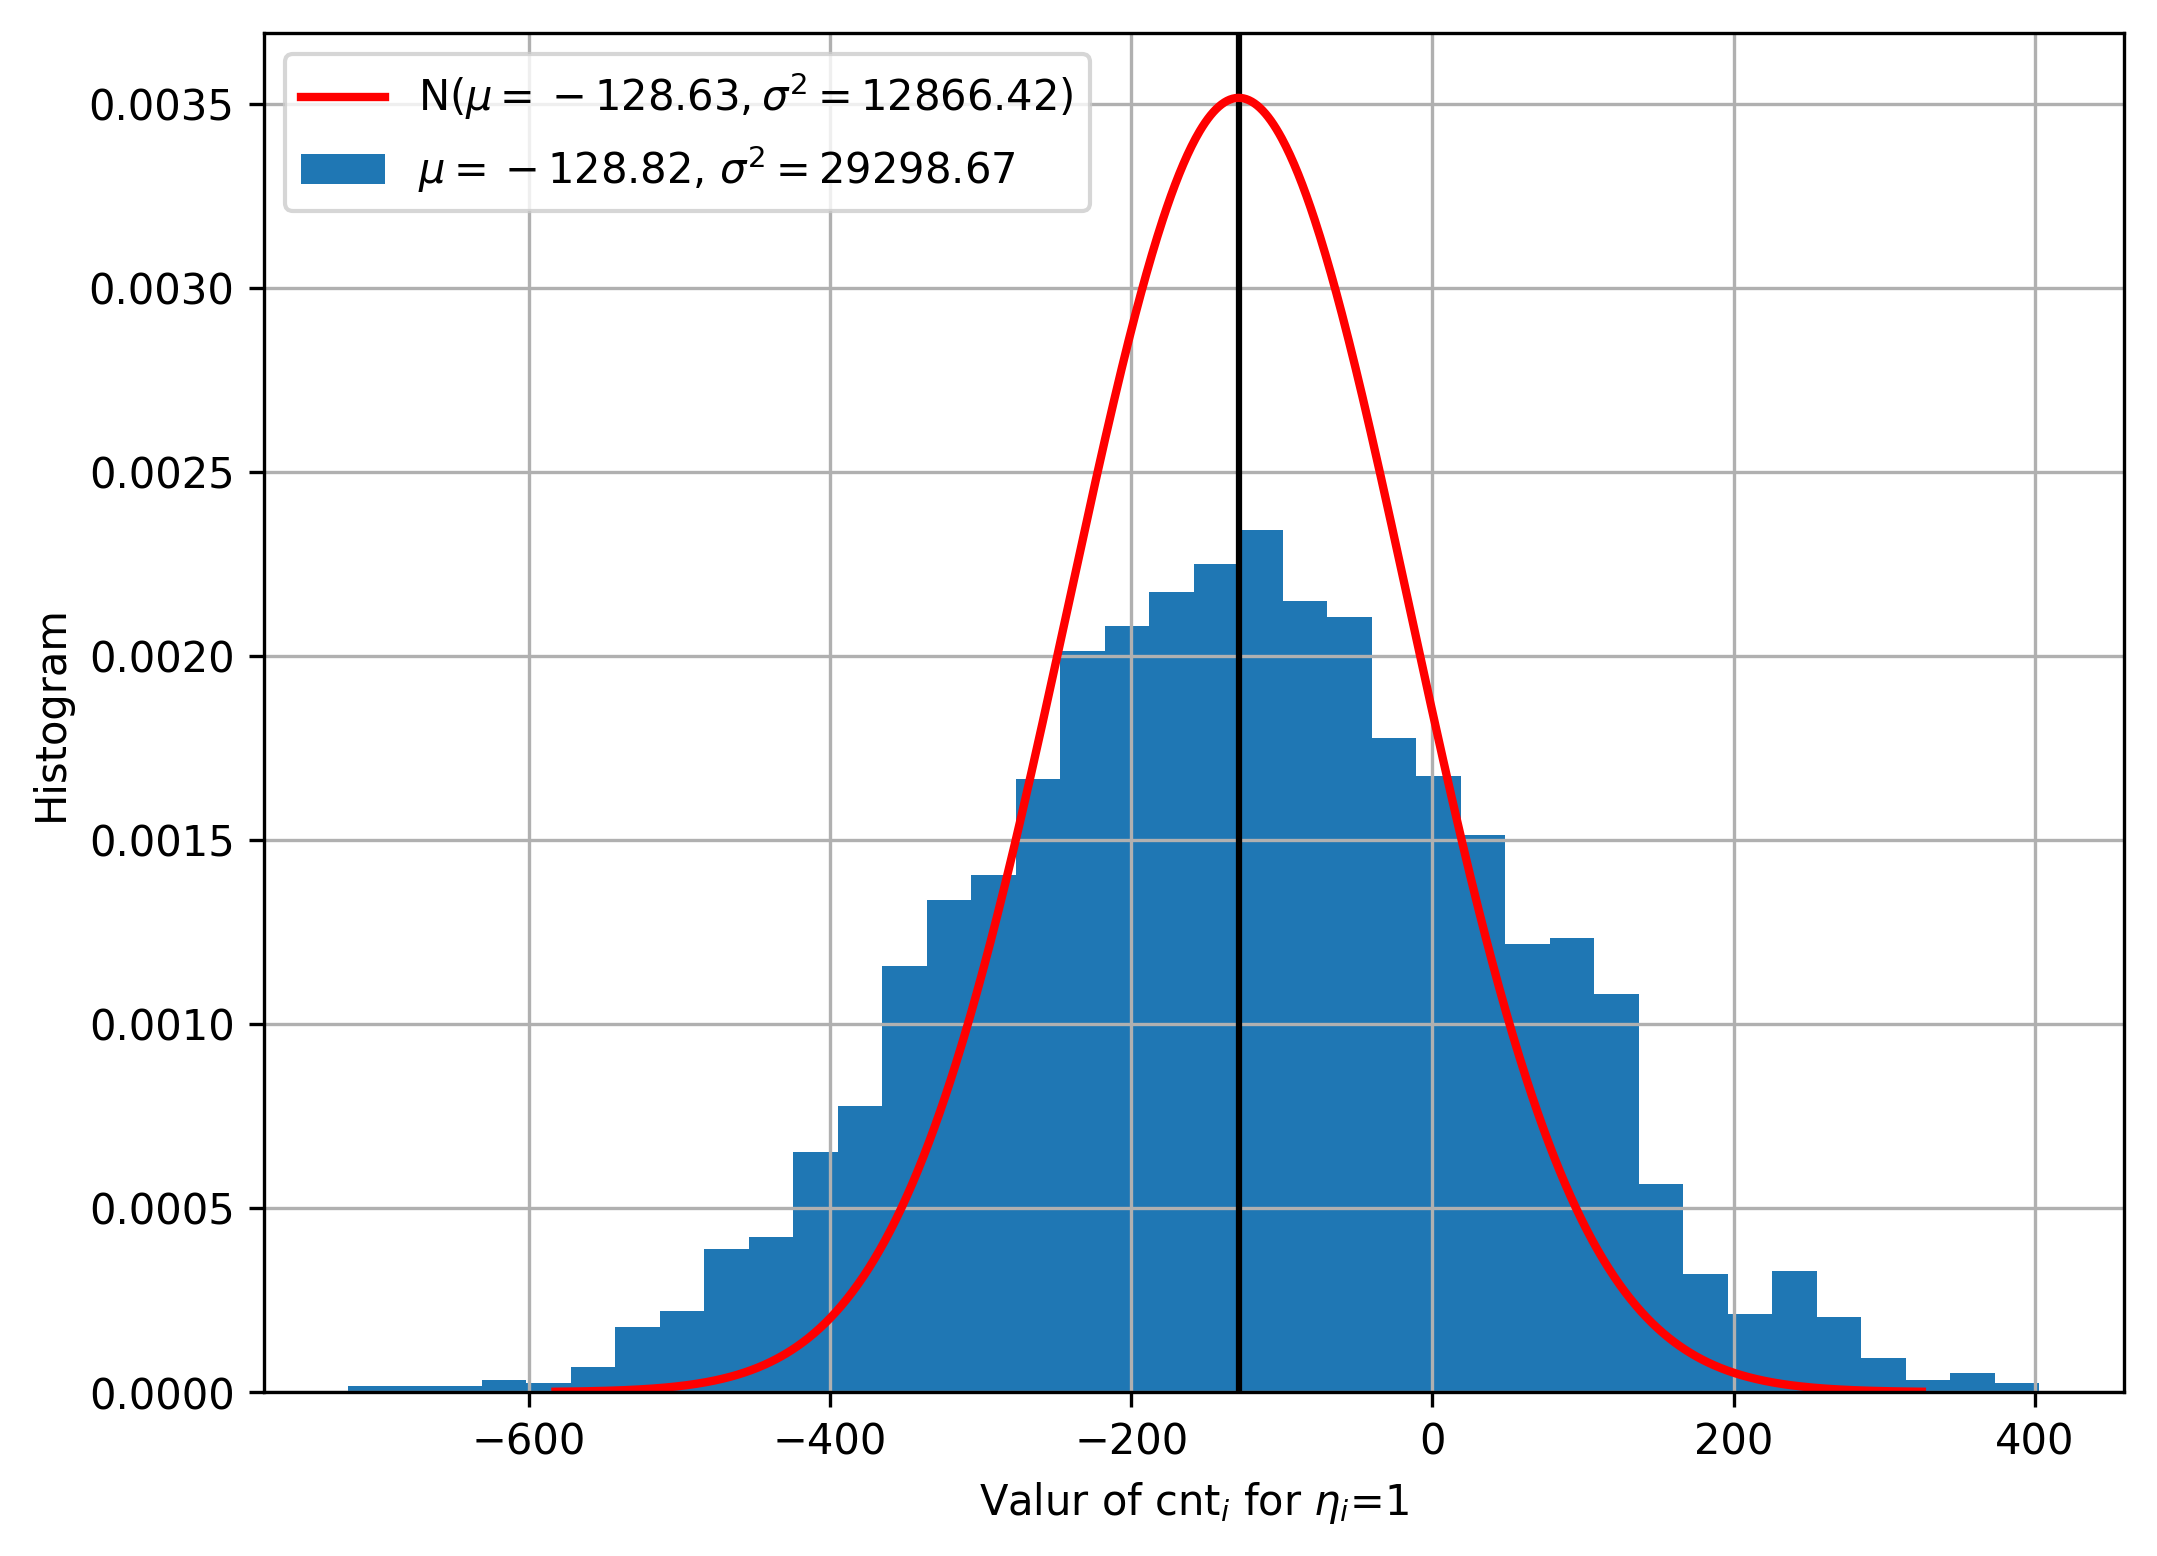
\includegraphics[width=0.5\textwidth]{./images02/autocorrelation/read-counters-eta0.png}}

  \caption{The histogram was obtained through simulation. The red curve is the theoretical normal distribution.}
  \label{fig:sdm-read}
\end{figure}


Finally,

\begin{align}
P(wrong) &= P(\text{acc}_i < 0 | \eta_i = 1) \cdot P(\eta_i = 1) + P(\text{acc}_i > 0 | \eta_i = 0) \cdot P(\eta_i = 0) \\
    &= \frac{\mathcal{N}_{\eta_i=1}.\text{cdf}(0)}{2} + \frac{1-\mathcal{N}_{\eta_i=0}.\text{cdf}(0)}{2} \\
    &= \frac{\mathcal{N}_{\eta_i=1}.\text{cdf}(0)}{2} + \frac{\mathcal{N}_{\eta_i=1}.\text{cdf}(0)}{2} \\
    &= \mathcal{N}_{\eta_i=1}.\text{cdf}(0)
\end{align}

Using the empirical variance of $\sigma^2 = 27838.3029124$, we calculate $P(wrong) = 0.22037771219874325$.

In order to check this probability, I have run a simulation reading from 1,000 random bitstrings (which have never been written into memory) and calculate the distance from the result of a single read. As the $P(wrong) = 0.22037$, I expected to get an average distance of 220.37 with a standard deviation of 13.10. See Figure \ref{fig:sdm-read-random-bs} for the comparison between the simulated and the theoretical outcomes.

Figure \ref{fig:sdm-single-read-dist} shows the new distance between $\eta_d$ and $\text{read}(\eta_d)$, where $\eta_d$ is $d$ bits away from $\eta$. As for $d \ge 520$ there is no intersection between $\eta$ and $\eta_d$, our models applies and explains the horizontal line around distance 220.

\begin{figure}[!htb]
  \centering
  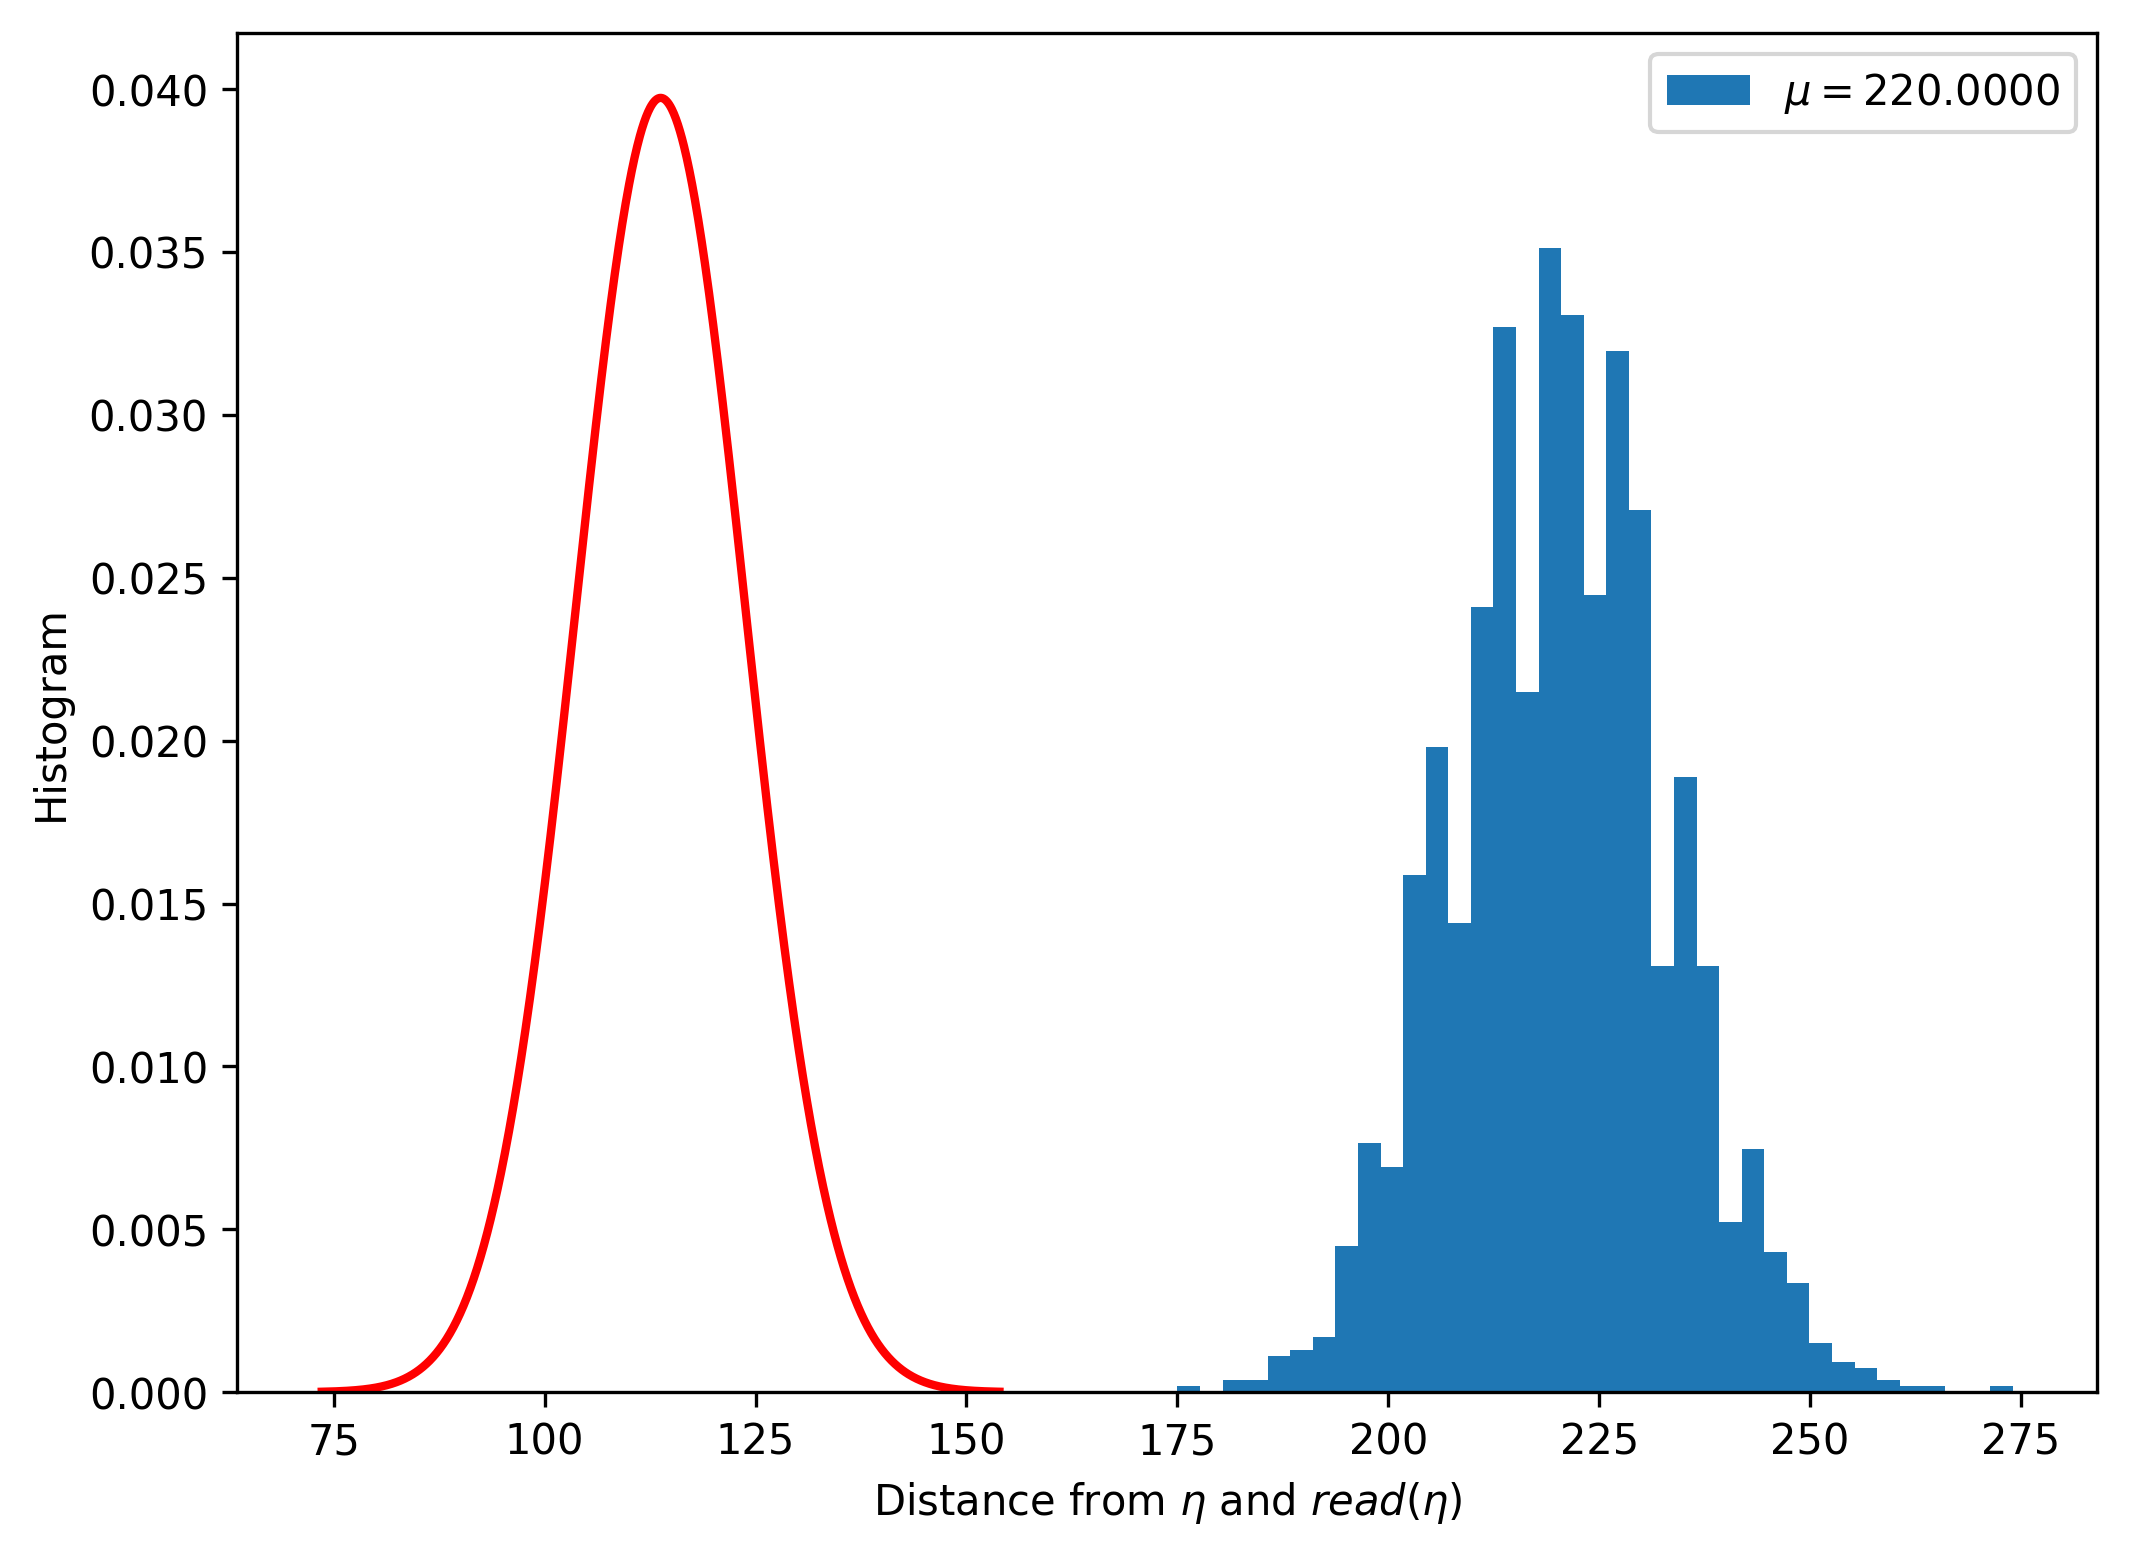
\includegraphics[width=0.6\textwidth]{./images02/autocorrelation/read-random-bs.png}

  \caption{The histogram was obtained through simulation. The red curve is the theoretical normal distribution.}
  \label{fig:sdm-read-random-bs}
\end{figure}

\begin{figure}[!htb]
  \centering
  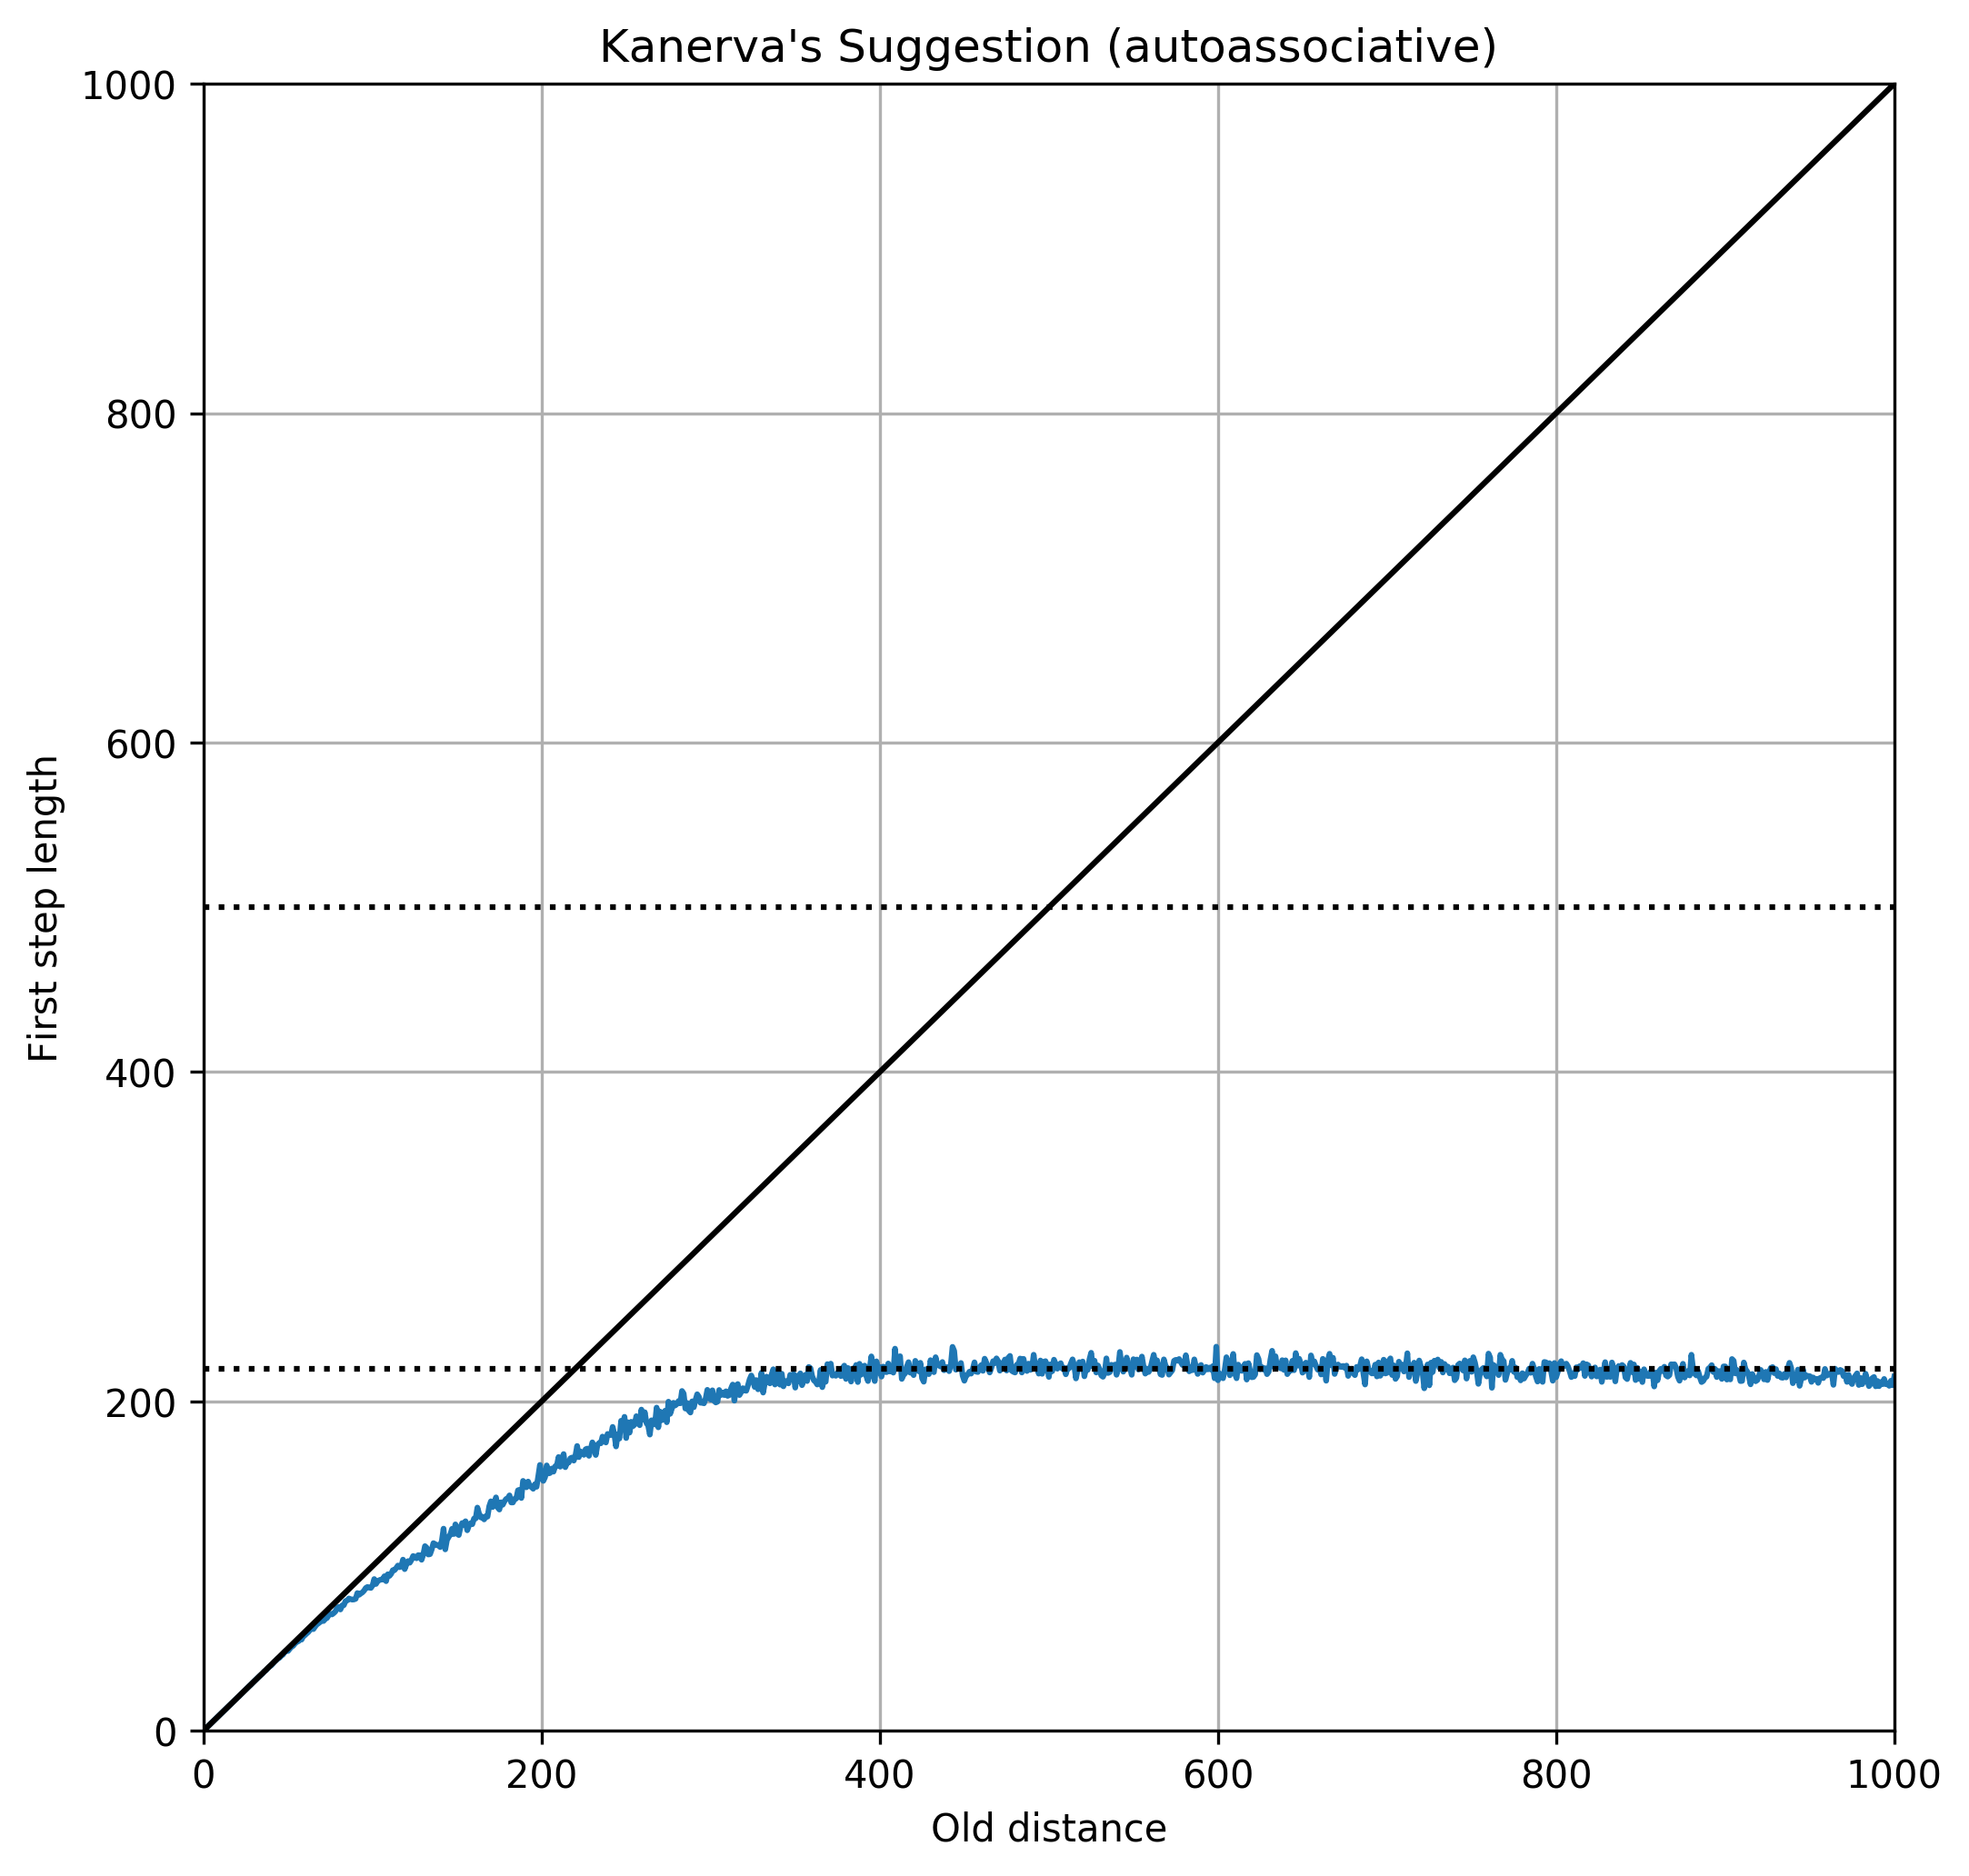
\includegraphics[width=0.6\textwidth]{./images02/autocorrelation/single-read-dist.png}

  \caption{New distance after a single read operation in a bitstring $\eta_d$, which is $d$ bits away from $\eta$. The new distance was calculated between $\eta_d$ and $\text{read}(\eta_d)$. Notice that when $d \ge 520$, the intersection between $\eta$ and $\eta_d$ is zero, which means there is only random bitstrings written into the activated hard locations. The distance 220 equals $1000 \cdot 0.220$ which is the probability find in Figure \ref{fig:sdm-read-random-bs}.}
  \label{fig:sdm-single-read-dist}
\end{figure}






% The very first letter is a 2 line initial drop letter followed
% by the rest of the first word in caps.
%
% form to use if the first word consists of a single letter:
% \IEEEPARstart{A}{demo} file is ....
%
% form to use if you need the single drop letter followed by
% normal text (unknown if ever used by the IEEE):
% \IEEEPARstart{A}{}demo file is ....
%
% Some journals put the first two words in caps:
% \IEEEPARstart{T}{his demo} file is ....
%
% Here we have the typical use of a "T" for an initial drop letter
% and "HIS" in caps to complete the first word.
\IEEEPARstart{S}{parse distributed memory} is a blha blha demo file is intended to serve as a ``starter file''
for IEEE journal papers produced under \LaTeX\ using
IEEEtran.cls version 1.8b and later.
% You must have at least 2 lines in the paragraph with the drop letter
% (should never be an issue)
I wish you the best of success.
Kanerva writes:




\section{A deviation from the equator distance?}

\begin{figure}[!htb]
\centering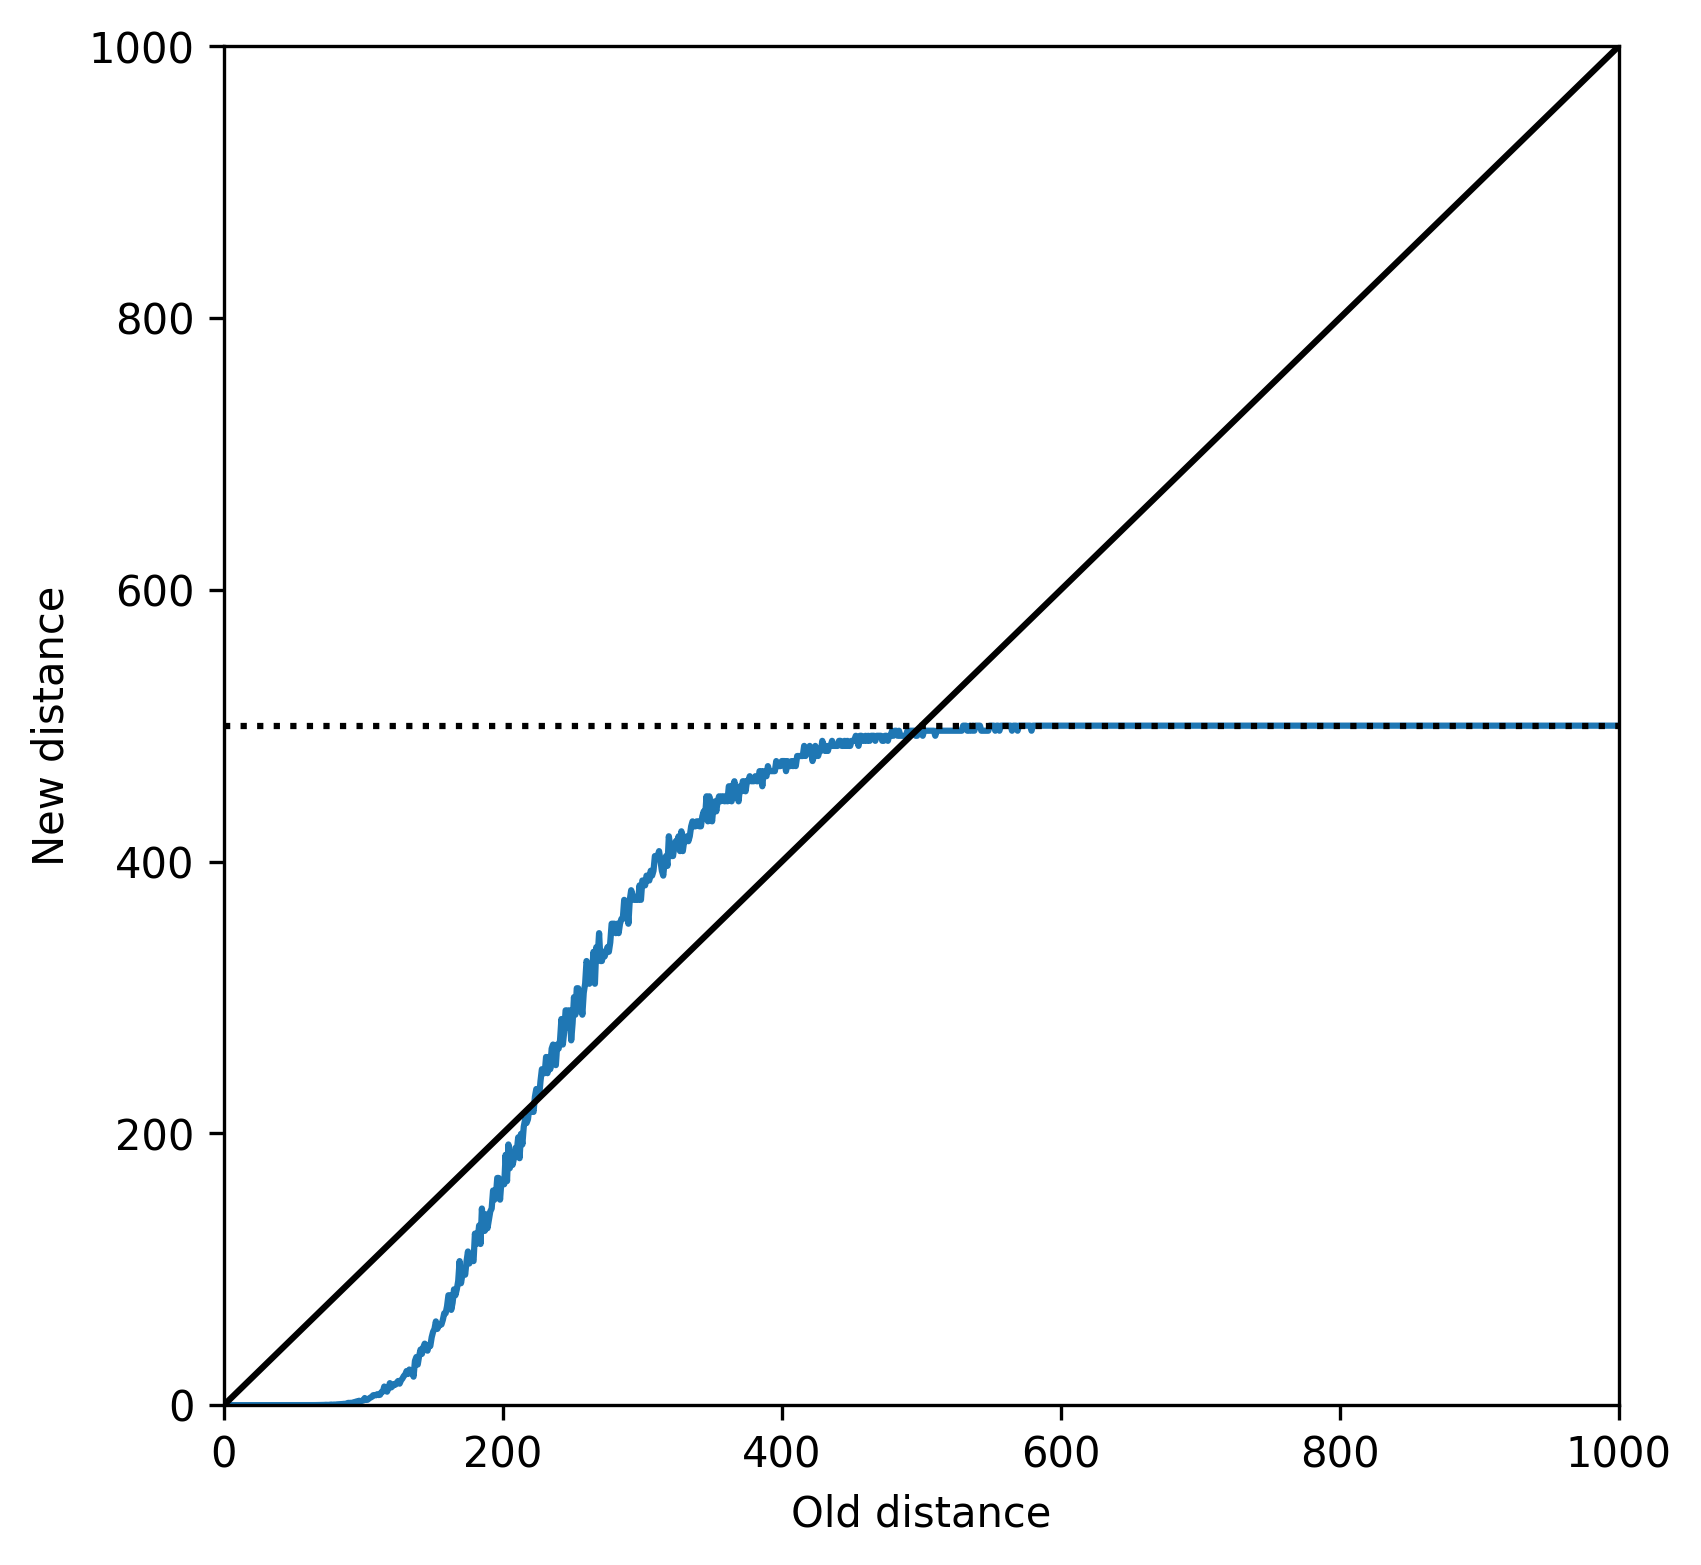
\includegraphics[width=0.8\textwidth]{./images02/calculated-table-72.png}
\caption{Kanerva's original Figure 7.3 generated using the equations from \citet{brogliato2014sparse}.
\label{fig:kanerva-figure-73-calculated}
}
\end{figure}



Kanerva writes:


    You have done an incredibly thorough analysis of SDM. I like the puzzle in your message and believe that your simulations are correct and to be learned from.  So what to make of the difference compared to my Figure 7.3 (and your Figure \ref{fig:kanerva-figure-73-calculated})?  I think the difference comes from my not having accounted fully for the effect of the other 9,999 vectors that are stored in the memory.  You say in it\\

   %``Our results show that the theoretical prediction is not accurate. There are interaction effects from one or more of the attractors created by the 10,000 writes, and these attractors seem to raise the distance beyond 500 bits (Figure \ref{fig:sdm-10000w-table-7-2}).'' \\

   I think that is correct.  It also brings to mind a comment Louis Jaeckel made when we worked at NASA Ames.  He pointed out that autoassociative storage (each vector is stored with itself as the address) introduces autocorrelation that my formula for Figure 7.2 did not take into account.  When we read from memory, each stored vector exerts a pull toward itself, which also means that each bit of a retrieved vector is slightly biased toward the same bit of the read address, regardless of the read address.  We never worked out the math.


This is an important observation. A hard location is activated because it shares many dimensions with the items read from or written onto it. Imagine the `counter's eye view':  each individual counter `likes' to write on its own corresponding bit-address value more than it likes the opposite; as each hard-location has a say in its own area --- and nowhere else.



Let $x$ and $y$ be random bitstrings and $n$ be the number of dimensions in the memory; let $x_i$ and $y_i$ be the $i$-th bit of $x$ and $y$, respectively; and $d(x, y)$ be the Hamming distance. Whilst the probability of a shared bit-value between same dimension-bits in two random addresses is $1/2$, an address only activates hard-locations close to it.  Let us call these shared bitvalues a \emph{bitmatch in dimension $i$}.

So, what is the probability of bitmatches given that we know the access radius $r$ between the address and a hard-location?
































\subsection{Subsection Heading Here}
Subsection text here.

% needed in second column of first page if using \IEEEpubid
%\IEEEpubidadjcol

\subsubsection{Subsubsection Heading Here}
Subsubsection text here.


% An example of a floating figure using the graphicx package.
% Note that \label must occur AFTER (or within) \caption.
% For figures, \caption should occur after the \includegraphics.
% Note that IEEEtran v1.7 and later has special internal code that
% is designed to preserve the operation of \label within \caption
% even when the captionsoff option is in effect. However, because
% of issues like this, it may be the safest practice to put all your
% \label just after \caption rather than within \caption{}.
%
% Reminder: the "draftcls" or "draftclsnofoot", not "draft", class
% option should be used if it is desired that the figures are to be
% displayed while in draft mode.
%
%\begin{figure}[!t]
%\centering
%\includegraphics[width=2.5in]{myfigure}
% where an .eps filename suffix will be assumed under latex,
% and a .pdf suffix will be assumed for pdflatex; or what has been declared
% via \DeclareGraphicsExtensions.
%\caption{Simulation results for the network.}
%\label{fig_sim}
%\end{figure}

% Note that the IEEE typically puts floats only at the top, even when this
% results in a large percentage of a column being occupied by floats.


% An example of a double column floating figure using two subfigures.
% (The subfig.sty package must be loaded for this to work.)
% The subfigure \label commands are set within each subfloat command,
% and the \label for the overall figure must come after \caption.
% \hfil is used as a separator to get equal spacing.
% Watch out that the combined width of all the subfigures on a
% line do not exceed the text width or a line break will occur.
%
%\begin{figure*}[!t]
%\centering
%\subfloat[Case I]{\includegraphics[width=2.5in]{box}%
%\label{fig_first_case}}
%\hfil
%\subfloat[Case II]{\includegraphics[width=2.5in]{box}%
%\label{fig_second_case}}
%\caption{Simulation results for the network.}
%\label{fig_sim}
%\end{figure*}
%
% Note that often IEEE papers with subfigures do not employ subfigure
% captions (using the optional argument to \subfloat[]), but instead will
% reference/describe all of them (a), (b), etc., within the main caption.
% Be aware that for subfig.sty to generate the (a), (b), etc., subfigure
% labels, the optional argument to \subfloat must be present. If a
% subcaption is not desired, just leave its contents blank,
% e.g., \subfloat[].


% An example of a floating table. Note that, for IEEE style tables, the
% \caption command should come BEFORE the table and, given that table
% captions serve much like titles, are usually capitalized except for words
% such as a, an, and, as, at, but, by, for, in, nor, of, on, or, the, to
% and up, which are usually not capitalized unless they are the first or
% last word of the caption. Table text will default to \footnotesize as
% the IEEE normally uses this smaller font for tables.
% The \label must come after \caption as always.
%
%\begin{table}[!t]
%% increase table row spacing, adjust to taste
%\renewcommand{\arraystretch}{1.3}
% if using array.sty, it might be a good idea to tweak the value of
% \extrarowheight as needed to properly center the text within the cells
%\caption{An Example of a Table}
%\label{table_example}
%\centering
%% Some packages, such as MDW tools, offer better commands for making tables
%% than the plain LaTeX2e tabular which is used here.
%\begin{tabular}{|c||c|}
%\hline
%One & Two\\
%\hline
%Three & Four\\
%\hline
%\end{tabular}
%\end{table}


% Note that the IEEE does not put floats in the very first column
% - or typically anywhere on the first page for that matter. Also,
% in-text middle ("here") positioning is typically not used, but it
% is allowed and encouraged for Computer Society conferences (but
% not Computer Society journals). Most IEEE journals/conferences use
% top floats exclusively.
% Note that, LaTeX2e, unlike IEEE journals/conferences, places
% footnotes above bottom floats. This can be corrected via the
% \fnbelowfloat command of the stfloats package.




\section{Conclusion}
The conclusion goes here.





% if have a single appendix:
%\appendix[Proof of the Zonklar Equations]
% or
%\appendix  % for no appendix heading
% do not use \section anymore after \appendix, only \section*
% is possibly needed

% use appendices with more than one appendix
% then use \section to start each appendix
% you must declare a \section before using any
% \subsection or using \label (\appendices by itself
% starts a section numbered zero.)
%


\appendices
\section{Proof of the First Zonklar Equation}
Appendix one text goes here.

% you can choose not to have a title for an appendix
% if you want by leaving the argument blank
\section{}
Appendix two text goes here.


% use section* for acknowledgment
\section*{Acknowledgment}


The authors would like to thank Pentti Kanerva, Eric Paul Nichols, José Ricardo de Almeida Torreão, Moacyr Alvim Horta Barbosa da Silva, Flavio Codeço Coelho, Horacio Hideki Yanasse, and Paulo Murillo for their careful, comprehensive, reviews of the first author's theses.


% Can use something like this to put references on a page
% by themselves when using endfloat and the captionsoff option.
\ifCLASSOPTIONcaptionsoff
  \newpage
\fi



% trigger a \newpage just before the given reference
% number - used to balance the columns on the last page
% adjust value as needed - may need to be readjusted if
% the document is modified later
%\IEEEtriggeratref{8}
% The "triggered" command can be changed if desired:
%\IEEEtriggercmd{\enlargethispage{-5in}}

% references section

% can use a bibliography generated by BibTeX as a .bbl file
% BibTeX documentation can be easily obtained at:
% http://mirror.ctan.org/biblio/bibtex/contrib/doc/
% The IEEEtran BibTeX style support page is at:
% http://www.michaelshell.org/tex/ieeetran/bibtex/
%\bibliographystyle{IEEEtran}
% argument is your BibTeX string definitions and bibliography database(s)
%\bibliography{IEEEabrv,../bib/paper}
%
% <OR> manually copy in the resultant .bbl file
% set second argument of \begin to the number of references
% (used to reserve space for the reference number labels box)
\begin{thebibliography}{1}

\bibitem{IEEEhowto:kopka}
H.~Kopka and P.~W. Daly, \emph{A Guide to \LaTeX}, 3rd~ed.\hskip 1em plus
  0.5em minus 0.4em\relax Harlow, England: Addison-Wesley, 1999.

\end{thebibliography}

% biography section
%
% If you have an EPS/PDF photo (graphicx package needed) extra braces are
% needed around the contents of the optional argument to biography to prevent
% the LaTeX parser from getting confused when it sees the complicated
% \includegraphics command within an optional argument. (You could create
% your own custom macro containing the \includegraphics command to make things
% simpler here.)
%\begin{IEEEbiography}[{\includegraphics[width=1in,height=1.25in,clip,keepaspectratio]{mshell}}]{Michael Shell}
% or if you just want to reserve a space for a photo:

\begin{IEEEbiography}{Michael Shell}
Biography text here.
\end{IEEEbiography}

% if you will not have a photo at all:
\begin{IEEEbiographynophoto}{John Doe}
Biography text here.
\end{IEEEbiographynophoto}

% insert where needed to balance the two columns on the last page with
% biographies
%\newpage

\begin{IEEEbiographynophoto}{Jane Doe}
Biography text here.
\end{IEEEbiographynophoto}

% You can push biographies down or up by placing
% a \vfill before or after them. The appropriate
% use of \vfill depends on what kind of text is
% on the last page and whether or not the columns
% are being equalized.

%\vfill

% Can be used to pull up biographies so that the bottom of the last one
% is flush with the other column.
%\enlargethispage{-5in}



% that's all folks
\end{document}
